\chapter{含参期望的梯度估计}
\label{chap:expectation-gradient-estimation}

设$X\sim\mathcal{N}(\theta,1)$，要计算$J(\theta)=\mathbb{E}[X^{2}]$对$\theta$的导数。这个例子有闭式答案$J(\theta)=\theta^{2}+1$，导数是$2\theta$。可是一旦分布或函数稍复杂，期望本身就只能用样本平均近似，导数也只能靠样本来算。一个自然的想法是把样本平均$\frac{1}{n}\sum_{i}X_{i}^{2}$对$\theta$求导；但$X_{i}^{2}$的表达式里看不到$\theta$，这样求出的导数是零。错在哪里？参数没有出现在函数里，却改变了样本从哪里来。

本章研究这类问题：含参期望$J(\bm{\theta})$等于$\mathbb{E}_{\bm{\theta}}[f_{\bm{\theta}}(X)]$，其中的参数既可能改变被积函数，也可能改变概率分布，怎样用随机样本计算$\nabla J(\bm{\theta})$，所得的估计在什么条件下无偏、方差有多大。第一步是看清参数从哪里进入期望，并把“导数能否移到期望里面”这件事化为一个可检验的控制条件。之后按参数进入的位置分三种处理：分布固定时直接对函数求导；分布可以写成固定噪声经过含参映射的结果时，沿样本的生成路径求导（重参数化）；两者都不方便时，对概率权重求导（得分函数估计），包括归一化常数未知的情形。

三种表示的期望相同，样本上的波动却可以相差很多，因此接着用第~\ref{chap:variance-reduction}章的控制变量与条件期望来降低梯度估计的方差。最后讨论样本来自近似生成器或有限步Markov链时，求出的到底是谁的梯度。全章反复使用开头的高斯例子：$X=\theta+\varepsilon$、$\varepsilon\sim\mathcal{N}(0,1)$、$f(x)=x^{2}$，手算时固定四个标准正态数$\varepsilon=0.3,-1.1,0.8,-0.4$，读者可以逐步复现。

\section{含参期望}
\label{sec:pgrad-parametric}

参数$\bm{\theta}\in\Theta\subseteq\mathbb{R}^{k}$对应一族概率分布$P_{\bm{\theta}}$和一族被积函数$f_{\bm{\theta}}$，记
\begin{equation}
  J(\bm{\theta})=\mathbb{E}_{\bm{\theta}}[f_{\bm{\theta}}(X)]=\int f_{\bm{\theta}}(x)\,P_{\bm{\theta}}(\mathrm{d}x),
  \label{eq:pgrad-J}
\end{equation}
其中$\mathbb{E}_{\bm{\theta}}$表示$X\sim P_{\bm{\theta}}$时的期望。称这样的$J$为\term{含参期望}（parameter-dependent expectation）。目标是用样本计算梯度$\nabla J(\bm{\theta})\in\mathbb{R}^{k}$。在动手构造估计之前，有两件事要先弄清：参数改变了期望里的哪些量，以及什么时候允许把求导移进期望。

\paragraph{参数进入期望的位置}

计算期望要做三件事：按某种规律产生样本，在样本处求函数值，再按概率加权平均。参数可以在其中任何一处起作用。图~\ref{fig:pgrad-three-entries}把三种位置并排画出。

\begin{BookInlineFigure}
  \centering
  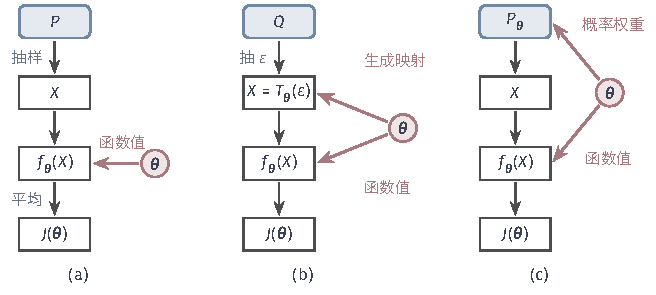
\includegraphics[width=111mm]{figures/07-probability/08-sampling-and-integration/tikz/pgrad-three-entries/figure.pdf}
  \caption{参数进入含参期望的三个位置。每列自上而下是随机性的来源、样本、函数值和期望；红色圆点标出参数进入之处。(a)抽样分布$P$固定，参数只改变函数值；(b)样本由固定分布$Q$的噪声$\varepsilon$经含参映射$T_{\bm{\theta}}$生成，参数既改变生成映射也改变函数；(c)参数改变分布$P_{\bm{\theta}}$本身，即改变各处的概率权重，同时也可以改变函数。}
  \label{fig:pgrad-three-entries}
\end{BookInlineFigure}

第一处是函数值：$f_{\bm{\theta}}(x)$在同一个$x$上随$\bm{\theta}$改变。第二处是概率权重：若$P_{\bm{\theta}}$有相对某个固定参考测度$\nu$的密度$p_{\bm{\theta}}$，参数改变的是各位置上的密度，即质量怎样分配。第三处是生成映射：样本写成$X=T_{\bm{\theta}}(\varepsilon)$，噪声$\varepsilon$的分布不变，参数改变的是同一个$\varepsilon$被送到哪里。

后两处描述的是同一件事的两种看法。对$X\sim\mathcal{N}(\theta,1)$，可以说“密度$p_{\theta}(x)=\varphi(x-\theta)$随$\theta$平移”，也可以说“$X=\theta+\varepsilon$，每个样本都向右挪了一段”。两种说法给出同一个分布族，计算梯度时只选一种，不能把分布的变化算两次。真正的要求是：在选定的表示里，凡是实际随参数变化的项都要计入，一项也不能漏。

\paragraph{两项相互抵消的例子}

取$X\sim\mathcal{N}(\theta,1)$与$f_{\theta}(x)=x^{2}-\theta x$。由$\mathbb{E}_{\theta}[X]=\theta$与$\mathbb{E}_{\theta}[X^{2}]=\theta^{2}+1$，得到
\[
  J(\theta)=\theta^{2}+1-\theta\cdot\theta=1 .
\]
$J$是常数，导数为零。现在把两种变化分开。固定分布在$\theta_{0}$，只让函数里的参数变成$t$，期望是
\[
  A(t)=\mathbb{E}_{\theta_{0}}[X^{2}-tX]=\theta_{0}^{2}+1-t\theta_{0},
\]
它在$t=\theta_{0}$处的斜率是$-\theta_{0}$。反过来固定函数为$f_{\theta_{0}}$，只让分布的参数变成$t$，期望是
\[
  B(t)=\mathbb{E}_{t}[X^{2}-\theta_{0}X]=t^{2}+1-\theta_{0}t,
\]
它在$t=\theta_{0}$处的斜率是$2\theta_{0}-\theta_{0}=\theta_{0}$。

两个斜率相加为零，正是$J'(\theta_{0})$。这就是二元函数$H(t_{1},t_{2})=\mathbb{E}_{t_{2}}[f_{t_{1}}(X)]$沿对角线$J(\theta)=H(\theta,\theta)$求导的链式法则（$H$在这里是多项式，可微性没有问题）。图~\ref{fig:pgrad-two-terms}在$\theta_{0}=1$处画出了三条曲线。只对函数求导会得到$-1$，只对分布求导会得到$+1$，两者都不是答案。

\begin{BookInlineFigure}
  \centering
  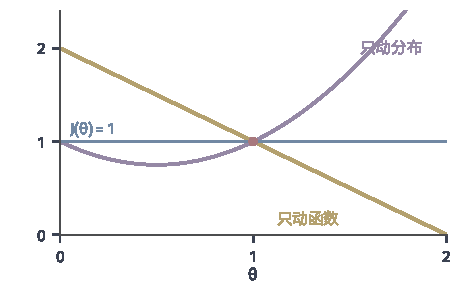
\includegraphics[width=78mm]{figures/07-probability/08-sampling-and-integration/matplotlib/pgrad-two-terms/figure.pdf}
  \caption{$X\sim\mathcal{N}(\theta,1)$，$f_{\theta}(x)=x^{2}-\theta x$。蓝线为$J(\theta)=1$；黄线为只让函数中的参数变化的$A(\theta)$；紫线为只让分布的参数变化的$B(\theta)$。三条线在红点$\theta=1$处相交，黄线斜率$-1$与紫线斜率$+1$之和等于蓝线斜率$0$。}
  \label{fig:pgrad-two-terms}
\end{BookInlineFigure}

\paragraph{期望在哪里有定义}

$J(\bm{\theta})$首先要有意义，即$f_{\bm{\theta}}$在$P_{\bm{\theta}}$下可积。例如$X\sim\operatorname{Exp}(1)$、$f_{\theta}(x)=\mathrm{e}^{\theta x}$时，
\[
  J(\theta)=\int_{0}^{\infty}\mathrm{e}^{\theta x}\mathrm{e}^{-x}\,\mathrm{d}x=\frac{1}{1-\theta},\qquad \theta<1,
\]
而$\theta\geq1$时积分发散。导数只在使$J$有定义的参数构成的开集内讨论：在某点求导，要求从该点出发朝每个方向走一小步，期望仍然有定义。因此下面总取一个以$\bm{\theta}_{0}$为中心、含在$\Theta$内的开球$U$，并检查$U$中每个参数下的可积性，而不只看$\bm{\theta}_{0}$这一点。

\paragraph{统一成固定测度上的积分}

三种参数位置可以写成同一种形式。图~\ref{fig:pgrad-three-entries}的三列分别对应
\[
  J(\bm{\theta})=\int f_{\bm{\theta}}\,\mathrm{d}P,\quad
  J(\bm{\theta})=\int f_{\bm{\theta}}(T_{\bm{\theta}}(\varepsilon))\,Q(\mathrm{d}\varepsilon),\quad
  J(\bm{\theta})=\int f_{\bm{\theta}}\,p_{\bm{\theta}}\,\mathrm{d}\nu .
\]
三个积分所对的测度$P$、$Q$、$\nu$都不随参数变化，参数全部被移进了被积函数。于是问题都化为：测度$\mu$固定，$g(\bm{\theta},x)$含参，
\begin{equation}
  J(\bm{\theta})=\int g(\bm{\theta},x)\,\mu(\mathrm{d}x)
  \label{eq:pgrad-fixed-measure}
\end{equation}
的梯度能否写成$\int\nabla_{\bm{\theta}}g(\bm{\theta},x)\,\mu(\mathrm{d}x)$。后面三节的区别只在于选哪个$\mu$和$g$，交换条件都由下面的定理检查。

\paragraph{交换的条件}

逐点可微只说明每个$x$上的函数$\bm{\theta}\mapsto g(\bm{\theta},x)$光滑，并不说明这些变化积分起来仍然受控：变化可能集中在越来越小的区域上，每个固定点都“看不到”它。需要一个与参数无关、可积的函数控制所有差商。

\begin{theorem}[积分号下求导]
\label{thm:pgrad-exchange}
设$\mu$是可测空间$\mathcal{X}$上的测度，$\bm{\theta}_{0}\in\Theta$，$U\subseteq\Theta$是以$\bm{\theta}_{0}$为中心的开球。设$g:U\times\mathcal{X}\to\mathbb{R}$满足：
\begin{enumerate}
  \item 对每个$\bm{\theta}\in U$，$g(\bm{\theta},\cdot)$可测，且$g(\bm{\theta}_{0},\cdot)$关于$\mu$可积；
  \item 对$\mu$几乎所有$x$，$\bm{\theta}\mapsto g(\bm{\theta},x)$在$\bm{\theta}_{0}$处可微；
  \item 存在$\mu$可积的函数$M\geq0$，使对$\mu$几乎所有$x$及所有$\bm{\theta},\bm{\theta}'\in U$，
  \begin{equation}
    \lvert g(\bm{\theta},x)-g(\bm{\theta}',x)\rvert\leq M(x)\lVert\bm{\theta}-\bm{\theta}'\rVert_{2}.
    \label{eq:pgrad-lipschitz}
  \end{equation}
\end{enumerate}
则对每个$\bm{\theta}\in U$，$g(\bm{\theta},\cdot)$可积，$\nabla_{\bm{\theta}}g(\bm{\theta}_{0},\cdot)$可积，式~\eqref{eq:pgrad-fixed-measure}的$J$在$\bm{\theta}_{0}$处可微，并且
\begin{equation}
  \nabla J(\bm{\theta}_{0})=\int\nabla_{\bm{\theta}}g(\bm{\theta}_{0},x)\,\mu(\mathrm{d}x).
  \label{eq:pgrad-exchange}
\end{equation}
\end{theorem}

\begin{proof}
先看可积性。由式~\eqref{eq:pgrad-lipschitz}取$\bm{\theta}'=\bm{\theta}_{0}$，对几乎所有$x$有
\[
  \lvert g(\bm{\theta},x)\rvert\leq\lvert g(\bm{\theta}_{0},x)\rvert+M(x)\lVert\bm{\theta}-\bm{\theta}_{0}\rVert_{2},
\]
右边可积，所以$g(\bm{\theta},\cdot)$可积，$J$在$U$上有定义。

再看梯度本身。记$\bm{v}(x)$为$g(\cdot,x)$在$\bm{\theta}_{0}$处的梯度，它的第$j$个分量是差商$\bigl(g(\bm{\theta}_{0}+h\bm{e}_{j},x)-g(\bm{\theta}_{0},x)\bigr)/h$沿$h=1/m\to0$的极限，是可测函数的极限，因而可测。由式~\eqref{eq:pgrad-lipschitz}，这些差商的绝对值都不超过$M(x)$，所以
\[
  \lVert\bm{v}(x)\rVert_{2}\leq\sqrt{k}\,M(x),
\]
$\bm{v}$可积。

最后证明可微。任取$\bm{h}_{m}\to\bm{0}$，$\bm{h}_{m}\neq\bm{0}$，$\bm{\theta}_{0}+\bm{h}_{m}\in U$，令
\[
  R_{m}(x)=\frac{g(\bm{\theta}_{0}+\bm{h}_{m},x)-g(\bm{\theta}_{0},x)-\langle\bm{v}(x),\bm{h}_{m}\rangle}{\lVert\bm{h}_{m}\rVert_{2}}.
\]
由条件2，对几乎所有$x$有$R_{m}(x)\to0$。由式~\eqref{eq:pgrad-lipschitz}与上一步的界，
\[
  \lvert R_{m}(x)\rvert\leq M(x)+\lVert\bm{v}(x)\rVert_{2}\leq(1+\sqrt{k})M(x).
\]
控制收敛定理给出$\int R_{m}\,\mathrm{d}\mu\to0$，也就是
\[
  \frac{J(\bm{\theta}_{0}+\bm{h}_{m})-J(\bm{\theta}_{0})-\bigl\langle\int\bm{v}\,\mathrm{d}\mu,\bm{h}_{m}\bigr\rangle}{\lVert\bm{h}_{m}\rVert_{2}}\to0 .
\]
序列$\bm{h}_{m}$是任取的，这正是$J$在$\bm{\theta}_{0}$处可微且梯度为$\int\bm{v}\,\mathrm{d}\mu$的定义。
\end{proof}

控制收敛定理的条件与证明可参考\BookChapterRef{chap:integration}{卷四第6章“积分”}。三个条件各管一件事。开球保证可以朝任意方向走一小步，并且沿线段比较。条件2只要求在$\bm{\theta}_{0}$这一点可微，例如$g(\theta,x)=\lvert\theta+x\rvert$在$\theta+x=0$处不可微，但对固定的$\theta_{0}$，这样的$x$只有一个，只要$\mu$在这一点没有质量，就不影响结论。条件3是关键：常数$M(x)$不能依赖参数，而且要对$x$可积。

常用的充分条件是梯度的一致控制。若对几乎所有$x$，$g(\cdot,x)$在整个$U$上可微，并且
\[
  \sup_{\bm{\theta}\in U}\lVert\nabla_{\bm{\theta}}g(\bm{\theta},x)\rVert_{2}\leq M(x),
\]
则沿连接$\bm{\theta}'$与$\bm{\theta}$的线段用中值定理，即得式~\eqref{eq:pgrad-lipschitz}。高斯族里的多项式函数就适合这样检查：参数限制在有界球内时，梯度不超过某个多项式乘以$\mathrm{e}^{-cx^{2}}$，后者可积。

\paragraph{逐点可微而交换失败}

下面的例子说明条件3不能省。取$U\sim\operatorname{Unif}(0,1)$，对$u\in(0,1)$令
\[
  g(\theta,u)=\frac{2\theta^{3}u}{(u^{2}+\theta^{2})^{2}},\qquad g(0,u)=0 .
\]
对每个固定的$u>0$，$g(\cdot,u)$是$\theta$的光滑函数。在$\theta=0$处，差商
\[
  \frac{g(\theta,u)-g(0,u)}{\theta}=\frac{2\theta^{2}u}{(u^{2}+\theta^{2})^{2}}\to0\qquad(\theta\to0),
\]
所以逐点导数为零，积分后仍是零。

另一方面，令$w=u^{2}+\theta^{2}$，$\mathrm{d}w=2u\,\mathrm{d}u$，对$\theta\neq0$有
\[
  J(\theta)=\theta^{3}\int_{\theta^{2}}^{1+\theta^{2}}w^{-2}\,\mathrm{d}w=\theta^{3}\Bigl(\frac{1}{\theta^{2}}-\frac{1}{1+\theta^{2}}\Bigr)=\frac{\theta}{1+\theta^{2}} .
\]
这个式子在$\theta=0$也成立，于是$J'(0)=1\neq0$。

失败的原因在图~\ref{fig:pgrad-moving-spike}(a)中一目了然。$g(\theta,\cdot)$是一个高度固定（约$0.65$）、宽度与$\theta$成正比的尖峰，$\theta\to0$时它被挤向$u=0$，面积约为$\theta$。每个固定的$u$最终都落在尖峰右侧，只看到函数值趋于零；尖峰携带的面积却以斜率$1$消失。用定理的语言说：对$\theta$求偏导数，
\[
  \partial_{\theta}g(\theta,u)=\frac{2u\bigl(3\theta^{2}(u^{2}+\theta^{2})-4\theta^{4}\bigr)}{(u^{2}+\theta^{2})^{3}},
\]
在$\theta=u$处它等于$1/(2u)$。任何满足式~\eqref{eq:pgrad-lipschitz}的$M$都要在$(0,\delta)$上不小于$1/(2u)$，而$\int_{0}^{\delta}\frac{1}{2u}\,\mathrm{d}u=\infty$。被积函数本身有界、逐点光滑，仍然不够。

\begin{BookInlineFigure}
  \centering
  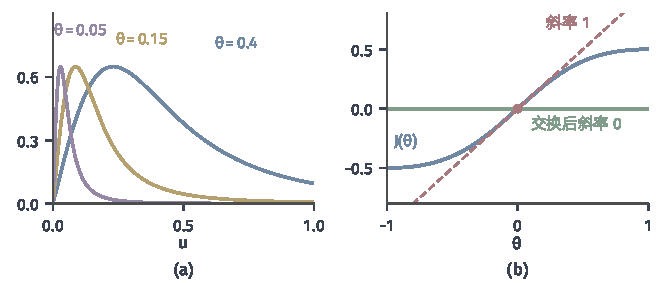
\includegraphics[width=112mm]{figures/07-probability/08-sampling-and-integration/matplotlib/pgrad-moving-spike/figure.pdf}
  \caption{逐点可微而不能交换求导与积分。(a)$g(\theta,u)=2\theta^{3}u/(u^{2}+\theta^{2})^{2}$在$\theta=0.4,0.15,0.05$时的图像，峰高都约为$0.65$，峰向$u=0$移动并变窄。(b)蓝线为$J(\theta)=\theta/(1+\theta^{2})$，红色虚线是它在原点处斜率为$1$的切线，绿线是逐点求导后再积分得到的斜率$0$。}
  \label{fig:pgrad-moving-spike}
\end{BookInlineFigure}

这个例子也说明了为什么检查要放在参数的一个邻域上，而不只在$\bm{\theta}_{0}$：在$\theta=0$这一点，每个$u$处的导数都存在且有界，毛病出在$\theta$离开零的过程中。后面每种梯度表示都先写成式~\eqref{eq:pgrad-fixed-measure}的形式，再用定理~\ref{thm:pgrad-exchange}检查。

\section{固定分布下的直接求导}
\label{sec:pgrad-direct}

最简单的情形是图~\ref{fig:pgrad-three-entries}(a)：抽样分布$P$与参数无关，参数只出现在函数里，$J(\bm{\theta})=\mathbb{E}_{P}[f_{\bm{\theta}}(X)]$。这时可以先在每个样本处对函数求导，再取平均吗？

\paragraph{梯度表示}

在定理~\ref{thm:pgrad-exchange}中取$\mu=P$、$g(\bm{\theta},x)=f_{\bm{\theta}}(x)$。若$f_{\bm{\theta}_{0}}$在$P$下可积，对$P$几乎所有$x$在$\bm{\theta}_{0}$处可微，并且在$\bm{\theta}_{0}$的某个开球$U$上满足式~\eqref{eq:pgrad-lipschitz}的可积控制，则
\begin{equation}
  \nabla J(\bm{\theta})=\mathbb{E}_{P}\bigl[\nabla_{\bm{\theta}}f_{\bm{\theta}}(X)\bigr].
  \label{eq:pgrad-direct}
\end{equation}
梯度本身成了一个期望，被积函数是逐样本的导数$\bm{G}=\nabla_{\bm{\theta}}f_{\bm{\theta}}(X)$。卷五的随机梯度方法就是在这种情形下使用样本梯度的，相应的交换引理可参考\BookChapterRef{chap:stochastic-gradient-methods}{卷五第13章“随机梯度方法”}。

\paragraph{样本估计}

取$X_{1},\dots,X_{n}$独立同分布于$P$，令
\begin{equation}
  \hat{\bm{g}}_{n}^{\mathrm{dir}}=\frac{1}{n}\sum_{i=1}^{n}\nabla_{\bm{\theta}}f_{\bm{\theta}}(X_{i}).
  \label{eq:pgrad-direct-estimator}
\end{equation}
这就是第~\ref{chap:monte-carlo-integration-error}章的样本平均，只不过被平均的是一个$\mathbb{R}^{k}$值函数。对它要问两件事，所需的条件不同。

第一件是期望与一致性。定理~\ref{thm:pgrad-exchange}的证明已经给出$\lVert\bm{G}\rVert_{2}\leq\sqrt{k}M(X)$，所以$\bm{G}$可积。由期望的线性，$\hat{\bm{g}}_{n}^{\mathrm{dir}}$的期望就是$\nabla J(\bm{\theta})$，估计无偏；对每个分量用强大数律（第~\ref{chap:laws-of-large-numbers}章），$\hat{\bm{g}}_{n}^{\mathrm{dir}}$几乎必然收敛到$\nabla J(\bm{\theta})$。这两条只用到一阶矩。

第二件是误差的大小。若$\mathbb{E}\lVert\bm{G}\rVert_{2}^{2}<\infty$，记$\bm{G}$的协方差矩阵为$\bm{\Sigma}_{\bm{G}}$，则各分量独立同分布平均的方差是$(\bm{\Sigma}_{\bm{G}})_{j,j}/n$，相加得到均方误差
\begin{equation}
  \mathbb{E}\bigl\lVert\hat{\bm{g}}_{n}^{\mathrm{dir}}-\nabla J(\bm{\theta})\bigr\rVert_{2}^{2}=\frac{\operatorname{tr}\bm{\Sigma}_{\bm{G}}}{n}.
  \label{eq:pgrad-direct-mse}
\end{equation}
这是熟悉的$n^{-1/2}$误差尺度。没有二阶矩时上式右边是无穷，大数律仍然成立，但误差缩小的速度可以慢得多。导数的可积性支撑“算得对”，导数的平方可积性才支撑“算得多准”。

\paragraph{一个只有一阶矩的例子}

设$X$的密度为$3x^{-4}$（$x\geq1$），$f_{\theta}(x)=x^{\theta}$。对$\theta<3$，
\[
  J(\theta)=\int_{1}^{\infty}x^{\theta}\cdot3x^{-4}\,\mathrm{d}x=\frac{3}{3-\theta},
\]
$\theta\geq3$时积分发散，所以只在$\theta<3$上讨论。逐样本导数是$G=X^{\theta}\ln X$。

先检查交换条件。取$\delta>0$使$\theta+\delta<3$，在$U=(\theta-\delta,\theta+\delta)$上
\[
  \bigl\lvert\partial_{\theta'}x^{\theta'}\bigr\rvert=x^{\theta'}\ln x\leq x^{\theta+\delta}\ln x,\qquad x\geq1,
\]
右边在$X$的分布下可积，因为
\[
  \int_{1}^{\infty}x^{\theta+\delta}\ln x\cdot3x^{-4}\,\mathrm{d}x=\frac{3}{(3-\theta-\delta)^{2}}<\infty .
\]于是由式~\eqref{eq:pgrad-direct}，
\[
  J'(\theta)=\mathbb{E}[X^{\theta}\ln X]=\frac{3}{(3-\theta)^{2}},
\]
与直接对$3/(3-\theta)$求导一致。

再看二阶矩。分部积分两次可得，对$a>1$，
\[
  \int_{1}^{\infty}x^{-a}\ln^{2}x\,\mathrm{d}x=\frac{2}{(a-1)^{3}} .
\]
取$a=4-2\theta$，得到
\[
  \mathbb{E}[G^{2}]=3\int_{1}^{\infty}x^{2\theta-4}\ln^{2}x\,\mathrm{d}x=\frac{6}{(3-2\theta)^{3}},\qquad\theta<\tfrac{3}{2},
\]
$\theta\geq\frac{3}{2}$时为无穷。在$\theta=1$处$J'(1)=\frac{3}{4}$，$\mathbb{E}[G^{2}]=6$，单样本方差$6-\frac{9}{16}=\frac{87}{16}\approx5.44$。在$\theta=2$处$J'(2)=3$，导数可积而方差无穷。

手算时用逆变换采样（第~\ref{chap:sample-generation}章）：分布函数是$1-x^{-3}$，于是$X=(1-U)^{-1/3}$。取均匀数$u=0.37,0.80,0.15,0.62$，得
\[
  X=1.1665,\ 1.7100,\ 1.0557,\ 1.3806 .
\]
在$\theta=1$处，四个导数样本$G=X\ln X$是
\[
  G=0.1797,\ 0.9174,\ 0.0572,\ 0.4453,
\]
平均为$0.3999$，真值是$0.75$。偏离约$0.35$，而四样本平均的标准差是$\sqrt{5.44/4}\approx1.17$，这个偏离在正常波动范围内。

图~\ref{fig:pgrad-pareto-paths}把样本数加到两万。$\theta=1$时各条路径在几百个样本后就贴近真值；$\theta=2$时路径长时间偏低，偶尔被一个巨大的样本拉高，然后再缓慢回落。这是无穷方差下的典型样子：绝大多数样本偏小，期望里相当一部分来自稀少的大值。

\begin{BookInlineFigure}
  \centering
  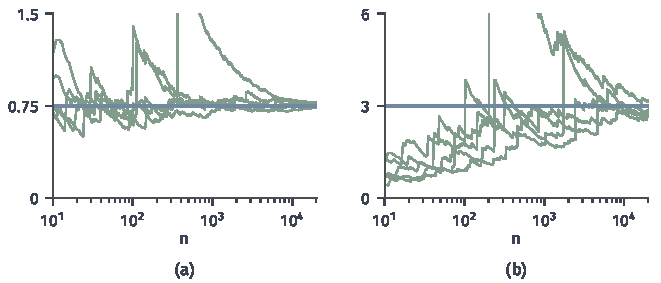
\includegraphics[width=112mm]{figures/07-probability/08-sampling-and-integration/matplotlib/pgrad-pareto-paths/figure.pdf}
  \caption{密度为$3x^{-4}$（$x\geq1$）时，导数样本$X^{\theta}\ln X$的运行平均，横轴为样本数$n$（对数刻度）。绿线为五条固定种子的独立路径，蓝线为真值$J'(\theta)=3/(3-\theta)^{2}$。(a)$\theta=1$，导数有有限方差；(b)$\theta=2$，导数可积但方差无穷。}
  \label{fig:pgrad-pareto-paths}
\end{BookInlineFigure}

图~\ref{fig:pgrad-pareto-error}量化了这种差别。对每个$n$重复$2000$次，取估计误差绝对值的中位数。$\theta=1$时误差沿$n^{-1/2}$的斜率下降，与式~\eqref{eq:pgrad-direct-mse}一致；$\theta=2$时下降明显更慢。这里$G$的尾部满足$\mathbb{P}(G>t)$约按$t^{-3/2}$（差一个对数因子）衰减，这类平均的误差尺度大约是$n^{-1/3}$。这一尺度来自重尾独立和的稳定极限，证明要用较细的特征函数估计，篇幅较长，读者可查阅~\scite{math-kallenberg2021probability}。图中$\theta=2$的折线在所示范围内甚至比这条参考线还平，对数因子在小样本时尤其明显。

\begin{BookInlineFigure}
  \centering
  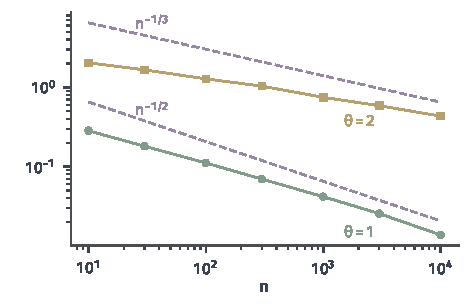
\includegraphics[width=80mm]{figures/07-probability/08-sampling-and-integration/matplotlib/pgrad-pareto-error/figure.pdf}
  \caption{同一例子中，$n$个导数样本平均的误差绝对值的中位数（每个$n$重复$2000$次，固定种子），双对数坐标。绿色圆点为$\theta=1$，黄色方块为$\theta=2$；紫色虚线是斜率为$-1/2$与$-1/3$的参考线。}
  \label{fig:pgrad-pareto-error}
\end{BookInlineFigure}

这个例子的教训适用于本章所有梯度估计：先用局部控制确认梯度可以写成期望，再单独检查梯度样本的二阶矩，二者不能互相代替。参数离可积性边界越近，导数样本的尾部越重，即使期望仍然有限，样本估计也会变得不可靠。

\section{重参数化估计}
\label{sec:pgrad-reparam}

回到章首的问题：$X\sim\mathcal{N}(\theta,1)$，$J(\theta)=\mathbb{E}[X^{2}]$。参数改变的是分布，上一节的方法不能直接用。但第~\ref{chap:sample-generation}章的生成方法提示了另一种写法：先抽$\varepsilon\sim\mathcal{N}(0,1)$，再令$X=\theta+\varepsilon$。噪声的分布与$\theta$无关，参数只出现在这个确定的映射里，于是分布的变化被改写成了函数的变化。

\paragraph{生成映射与梯度表示}

一般地，设噪声$\varepsilon$取值于某个空间、分布为$Q$且不依赖参数，$T_{\bm{\theta}}$是从噪声到$\mathbb{R}^{d}$的映射，使$T_{\bm{\theta}}(\varepsilon)$的分布正是$P_{\bm{\theta}}$，即$P_{\bm{\theta}}$是$Q$在$T_{\bm{\theta}}$下的推前。这样的写法称为\term{重参数化}（reparameterization）。由推前的换元公式，
\begin{equation}
  J(\bm{\theta})=\mathbb{E}_{Q}\bigl[f_{\bm{\theta}}(T_{\bm{\theta}}(\varepsilon))\bigr].
  \label{eq:pgrad-reparam-J}
\end{equation}
期望所对的分布$Q$固定，形式上回到了上一节：在定理~\ref{thm:pgrad-exchange}中取$\mu=Q$，以式~\eqref{eq:pgrad-reparam-J}方括号内的复合函数作$g(\bm{\theta},\varepsilon)$即可。

对固定的$\varepsilon$求$g$对$\bm{\theta}$的导数，要用链式法则。设$f_{\bm{\theta}}(x)$对$(\bm{\theta},x)$连续可微，$T_{\bm{\theta}}(\varepsilon)$对$\bm{\theta}$可微，记$x=T_{\bm{\theta}}(\varepsilon)$，$D_{\bm{\theta}}T_{\bm{\theta}}(\varepsilon)$为$d\times k$的Jacobi矩阵。参数沿两条路到达函数值：一条直接进入$f_{\bm{\theta}}$，另一条先移动样本点$x$，再经$f_{\bm{\theta}}$对$x$的梯度传到函数值。两条路的贡献相加，
\begin{equation}
  \nabla_{\bm{\theta}}\bigl[f_{\bm{\theta}}(T_{\bm{\theta}}(\varepsilon))\bigr]
  =\nabla_{\bm{\theta}}f_{\bm{\theta}}(x)+\bigl(D_{\bm{\theta}}T_{\bm{\theta}}(\varepsilon)\bigr)^{\top}\nabla_{x}f_{\bm{\theta}}(x).
  \label{eq:pgrad-chain}
\end{equation}
图~\ref{fig:pgrad-chain-paths}画出这两条路。称它为沿样本生成路径的导数，即\term{路径导数}（pathwise derivative）。

\begin{BookInlineFigure}
  \centering
  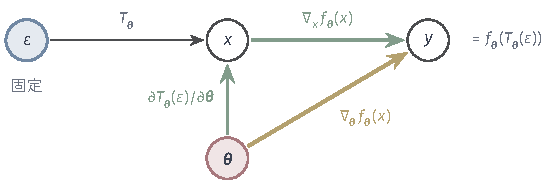
\includegraphics[width=94mm]{figures/07-probability/08-sampling-and-integration/tikz/pgrad-chain-paths/figure.pdf}
  \caption{一个重参数化样本的计算图。噪声$\varepsilon$（蓝）固定，参数$\bm{\theta}$（红）经两条路影响函数值$y$：黄色箭头是函数自身对参数的导数，绿色箭头是先经生成映射移动样本点、再经函数对$x$的梯度传递的部分。路径导数是两部分之和。}
  \label{fig:pgrad-chain-paths}
\end{BookInlineFigure}

把这些条件合起来，就得到重参数化的梯度表示。

\begin{theorem}[重参数化梯度]
\label{thm:pgrad-reparam}
设$P_{\bm{\theta}}$是$Q$在$T_{\bm{\theta}}$下的推前，$U$是以$\bm{\theta}_{0}$为中心的开球，复合函数$g(\bm{\theta},\varepsilon)$等于$f_{\bm{\theta}}(T_{\bm{\theta}}(\varepsilon))$。设对$Q$几乎所有$\varepsilon$，$\bm{\theta}\mapsto T_{\bm{\theta}}(\varepsilon)$在$\bm{\theta}_{0}$处可微，$(\bm{\theta},x)\mapsto f_{\bm{\theta}}(x)$在$(\bm{\theta}_{0},T_{\bm{\theta}_{0}}(\varepsilon))$的某个邻域内连续可微；又设$g$满足定理~\ref{thm:pgrad-exchange}的条件1与条件3（取$\mu=Q$）。记$X=T_{\bm{\theta}_{0}}(\varepsilon)$，则
\begin{equation}
  \nabla J(\bm{\theta}_{0})=\mathbb{E}_{Q}\Bigl[\nabla_{\bm{\theta}}f_{\bm{\theta}_{0}}(X)+\bigl(D_{\bm{\theta}}T_{\bm{\theta}_{0}}(\varepsilon)\bigr)^{\top}\nabla_{x}f_{\bm{\theta}_{0}}(X)\Bigr].
  \label{eq:pgrad-reparam}
\end{equation}
\end{theorem}

证明就是定理~\ref{thm:pgrad-exchange}本身。所设的可微性使链式法则对几乎所有$\varepsilon$成立，于是$g(\cdot,\varepsilon)$在$\bm{\theta}_{0}$处可微，梯度由式~\eqref{eq:pgrad-chain}给出，这正是定理~\ref{thm:pgrad-exchange}的条件2；再由式~\eqref{eq:pgrad-exchange}，$J$的梯度等于这些逐点梯度关于$Q$的积分。对独立的$\varepsilon_{1},\dots,\varepsilon_{n}\sim Q$，令$X_{i}=T_{\bm{\theta}}(\varepsilon_{i})$，\term{重参数化估计}（reparameterization gradient estimator）是式~\eqref{eq:pgrad-reparam}方括号内的量在这$n$个样本上的平均，记作$\hat{\bm{g}}_{n}^{\mathrm{rep}}$。无偏性、一致性与均方误差的讨论与上一节完全相同。

\paragraph{高斯的平移与尺度}

最常用的生成映射是高斯的位置尺度变换$X=\mu+\sigma\varepsilon$，$\varepsilon\sim\mathcal{N}(0,1)$，参数$\bm{\theta}=(\mu,\sigma)$，$\sigma>0$。映射对参数的导数是
\[
  \frac{\partial X}{\partial\mu}=1,\qquad\frac{\partial X}{\partial\sigma}=\varepsilon .
\]
增大$\mu$时每个样本平移同样的距离；增大$\sigma$时每个样本沿远离$\mu$的方向移动，移动量与它的$\varepsilon$成正比，$\varepsilon$为负的样本向左走，为正的向右走。图~\ref{fig:pgrad-reparam-map}用四个固定的$\varepsilon$画出了这两种移动。

\begin{BookInlineFigure}
  \centering
  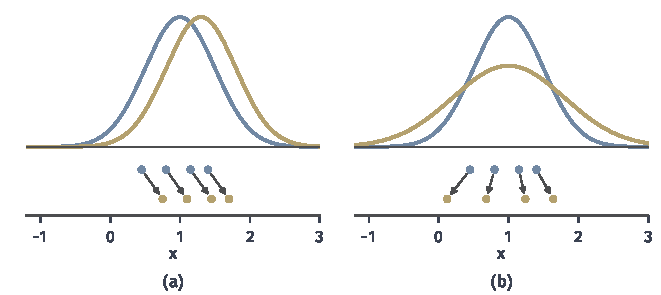
\includegraphics[width=112mm]{figures/07-probability/08-sampling-and-integration/matplotlib/pgrad-reparam-map/figure.pdf}
  \caption{高斯位置尺度变换下同一组噪声$\varepsilon=0.3,-1.1,0.8,-0.4$的样本怎样移动。蓝线与蓝点为$(\mu,\sigma)=(1,0.5)$时的密度与样本，黄线与黄点为参数改变后的密度与样本，箭头连接同一个$\varepsilon$生成的两个样本。(a)$\mu$由$1$变为$1.3$，各样本平移$0.3$；(b)$\sigma$由$0.5$变为$0.8$，样本$i$移动$0.3\varepsilon_{i}$。}
  \label{fig:pgrad-reparam-map}
\end{BookInlineFigure}

取$f(x)=x^{2}$，$J(\mu,\sigma)=\mu^{2}+\sigma^{2}$，梯度是$(2\mu,2\sigma)$。函数不含参数，式~\eqref{eq:pgrad-chain}只剩生成映射一项，两个分量的路径导数分别为
\[
  G_{\mu}=2X,\qquad G_{\sigma}=2X\varepsilon .
\]
由$\mathbb{E}[\varepsilon]=0$与$\mathbb{E}[\varepsilon^{2}]=1$，它们的期望是
\[
  \mathbb{E}[2X]=2\mu,\qquad\mathbb{E}[2(\mu+\sigma\varepsilon)\varepsilon]=2\sigma,
\]
与真值一致。交换条件也容易验证：参数限制在$\lvert\mu'-\mu\rvert<\delta$、$\lvert\sigma'-\sigma\rvert<\delta$内时，
\[
  \lvert G_{\mu}\rvert+\lvert G_{\sigma}\rvert\leq2\bigl(\lvert\mu\rvert+\delta+(\sigma+\delta)\lvert\varepsilon\rvert\bigr)(1+\lvert\varepsilon\rvert),
\]
右边是$\lvert\varepsilon\rvert$的二次多项式，在标准正态下可积。

下面用固定的噪声手算一次。取$(\mu,\sigma)=(1,0.5)$与$\varepsilon=0.3,-1.1,0.8,-0.4$，样本是
\[
  X=1.15,\ 0.45,\ 1.40,\ 0.80 .
\]
$\mu$分量的四个路径导数及其平均为
\[
  G_{\mu}=2.30,\ 0.90,\ 2.80,\ 1.60,\qquad\hat{g}_{\mu}=1.900,
\]
真值是$2$。$\sigma$分量为
\[
  G_{\sigma}=0.69,\ -0.99,\ 2.24,\ -0.64,\qquad\hat{g}_{\sigma}=0.325,
\]
真值是$1$。

$\sigma$分量偏得多，这不是计算错误。两个分量的单样本方差是
\[
  \operatorname{Var}(2X)=4\sigma^{2}=1,\qquad\operatorname{Var}(2X\varepsilon)=\operatorname{Var}(2\mu\varepsilon+2\sigma\varepsilon^{2})=4\mu^{2}+8\sigma^{2}=6,
\]
其中用到$\varepsilon$与$\varepsilon^{2}$的协方差$\mathbb{E}[\varepsilon^{3}]$为零，以及$\operatorname{Var}(\varepsilon^{2})=2$。四样本平均下$\sigma$分量的标准差约为$\sqrt{6/4}\approx1.22$，偏离$0.675$完全正常。同一个估计的不同分量，精度可以差很多。

\paragraph{函数自身与生成映射的贡献}

当函数也含参数时，式~\eqref{eq:pgrad-chain}的两项都出现。回到第~\ref{sec:pgrad-parametric}节的例子：$X=\theta+\varepsilon$，$f_{\theta}(x)=x^{2}-\theta x$。两条路的贡献分别是
\[
  \partial_{\theta}f_{\theta}(x)=-x,\qquad\partial_{x}f_{\theta}(x)\cdot\partial_{\theta}X=(2x-\theta)\cdot1 .
\]
两者相加，
\[
  \frac{\mathrm{d}}{\mathrm{d}\theta}f_{\theta}(\theta+\varepsilon)=-X+(2X-\theta)=X-\theta=\varepsilon,
\]
期望为零，与$J(\theta)=1$一致。单独取第一项得到$\mathbb{E}[-X]=-\theta$，单独取第二项得到$\mathbb{E}[2X-\theta]=\theta$，正是图~\ref{fig:pgrad-two-terms}中黄线与紫线的斜率。重参数化把“分布的变化”具体化成了“样本点的移动”，两项各有清楚的来源。

\paragraph{离散选择与不连续的生成步骤}

重参数化要求对每个固定的噪声，函数值随参数连续地、可控地变化。离散选择破坏了这一点。设$X\sim\operatorname{Bern}(\theta)$，用逆变换写成$X=\mathbf{1}_{\{U\leq\theta\}}$，$U\sim\operatorname{Unif}(0,1)$。对任意函数$f$，
\[
  J(\theta)=\theta f(1)+(1-\theta)f(0),\qquad J'(\theta)=f(1)-f(0).
\]
但对每个$U\neq\theta$，$X$在$\theta$附近是常数，路径导数为零，平均起来还是零。

图~\ref{fig:pgrad-bernoulli-threshold}说明了导数藏在哪里。参数从$\theta$增加到$\theta+h$时，只有落在$(\theta,\theta+h]$里的$U$使$X$由$0$跳到$1$，这件事的概率是$h$，每次跳跃使函数值改变$f(1)-f(0)$。期望的变化$h\bigl(f(1)-f(0)\bigr)$全部来自这些跳跃，而对任何固定的$U$，跳跃只发生在一个参数值上，逐点求导看不到它。用定理~\ref{thm:pgrad-exchange}的语言说，$g(\theta,u)=f(\mathbf{1}_{\{u\leq\theta\}})$在$\theta$的任何邻域内都有跳跃的$u$构成正概率集合，式~\eqref{eq:pgrad-lipschitz}不可能成立。

\begin{BookInlineFigure}
  \centering
  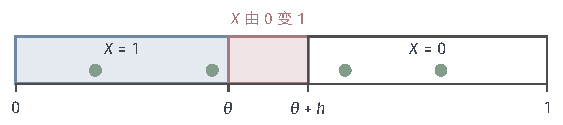
\includegraphics[width=96mm]{figures/07-probability/08-sampling-and-integration/tikz/pgrad-bernoulli-threshold/figure.pdf}
  \caption{用$X=\mathbf{1}_{\{U\leq\theta\}}$生成$\operatorname{Bern}(\theta)$。横轴是$U$的取值；蓝色区间上$X=1$。参数由$\theta=0.4$增至$\theta+h=0.55$时，只有红色区间内的$U$使$X$由$0$变为$1$，其概率为$h$。绿点是四个固定均匀数$0.37,0.80,0.15,0.62$，都不在红色区间内，它们生成的样本对参数的路径导数都是零。}
  \label{fig:pgrad-bernoulli-threshold}
\end{BookInlineFigure}

连续分布配上不连续的函数也会出同样的问题。取$f(x)=\mathbf{1}_{\{x>0\}}$，$X=\theta+\varepsilon$，则
\[
  J(\theta)=\mathbb{P}(\varepsilon>-\theta)=\Phi(\theta),\qquad J'(\theta)=\varphi(\theta)>0 .
\]对每个$\varepsilon\neq-\theta$，$f(\theta+\varepsilon)$在$\theta$附近是常数，路径导数为零。图~\ref{fig:pgrad-step-path}(a)中，四个固定噪声对应的平均$\frac{1}{4}\sum_{i}\mathbf{1}_{\{\theta+\varepsilon_{i}>0\}}$是一条阶梯，它逐段水平，导数只在台阶处“集中”。普通链式法则在这里不能直接沿用。

\begin{BookInlineFigure}
  \centering
  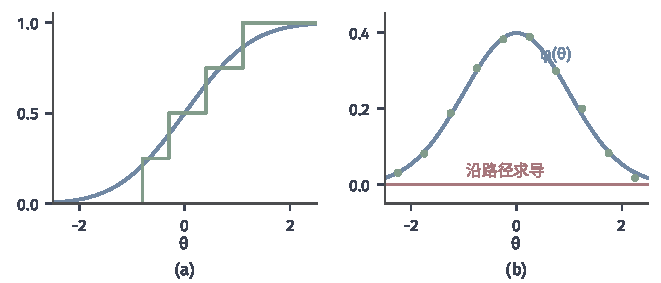
\includegraphics[width=112mm]{figures/07-probability/08-sampling-and-integration/matplotlib/pgrad-step-path/figure.pdf}
  \caption{$f(x)=\mathbf{1}_{\{x>0\}}$，$X=\theta+\varepsilon$。(a)蓝线为$J(\theta)=\Phi(\theta)$，绿色阶梯为四个固定噪声$\varepsilon=0.3,-1.1,0.8,-0.4$给出的样本平均，逐段水平。(b)蓝线为$J'(\theta)=\varphi(\theta)$，红线为路径导数的平均$0$，绿点为下一节得分函数估计在各$\theta$处的平均（每点$20000$个固定种子样本）。}
  \label{fig:pgrad-step-path}
\end{BookInlineFigure}

处理这类问题有三条出路。第一条是不对函数求导，改为对概率权重求导，这就是下一节的得分函数估计，图~\ref{fig:pgrad-step-path}(b)的绿点显示它在这个例子里给出正确的导数。第二条是把跳跃的贡献单独算出来：上例中$\frac{\mathrm{d}}{\mathrm{d}\theta}\mathbb{P}(\varepsilon>-\theta)$等于边界$\varepsilon=-\theta$处的密度，这一项可以解析地加回去。第三条是用光滑函数近似跳跃，再对近似求路径导数；这样得到的是近似问题的梯度，与原梯度的差需要另外控制。无论哪一条，都要先承认路径导数在这里不是原梯度的无偏估计。

不连续不等于不可用。若$f$是Lipschitz函数，例如$f(x)=\lvert x\rvert$，则由三角不等式
\[
  \bigl\lvert f(\theta+\varepsilon)-f(\theta'+\varepsilon)\bigr\rvert\leq\lvert\theta-\theta'\rvert,
\]
式~\eqref{eq:pgrad-lipschitz}以$M\equiv1$成立；不可微点$\theta+\varepsilon=0$只对一个$\varepsilon$出现，概率为零。于是路径导数$\operatorname{sign}(X)$的期望就是$J'(\theta)$。区分的标准不是“处处可微”，而是函数值随参数的变化能否被一个可积的Lipschitz常数控制。


\section{得分函数估计}
\label{sec:pgrad-score}

上一节最后的两个例子里，样本沿生成路径的变化是跳跃式的，路径导数看不到期望的变化。还有一些情形根本没有方便的生成映射，例如样本由Markov链产生。这时可以换一个角度：不跟踪样本点怎样移动，而看各位置的概率权重怎样变化。参数改变时，有的位置质量增加，有的减少；把函数值按这种增减加权求和，就是期望的变化率。第~\ref{chap:information-geometry}章的得分函数正好记录了每个位置上质量的相对变化率。

本节先处理密度可以完整计算的情形，再处理只知道密度到一个随参数变化的常数因子的情形。

\subsection{已归一化密度}
\label{sec:pgrad-score-normalized}

设$P_{\bm{\theta}}$相对固定的参考测度$\nu$有密度$p_{\bm{\theta}}$，支撑$S=\{x:p_{\bm{\theta}}(x)>0\}$不随$\bm{\theta}$改变。在$S$上，得分函数是
\[
  \bm{s}_{\bm{\theta}}(x)=\nabla_{\bm{\theta}}\ln p_{\bm{\theta}}(x)=\frac{\nabla_{\bm{\theta}}p_{\bm{\theta}}(x)}{p_{\bm{\theta}}(x)} .
\]
把期望写成参考测度上的积分
\[
  J(\bm{\theta})=\int_{S}f_{\bm{\theta}}\,p_{\bm{\theta}}\,\mathrm{d}\nu,
\]
在定理~\ref{thm:pgrad-exchange}中取$\mu$为$\nu$在$S$上的限制，以乘积$f_{\bm{\theta}}p_{\bm{\theta}}$作$g$。乘积的导数是
\[
  \nabla_{\bm{\theta}}(f_{\bm{\theta}}p_{\bm{\theta}})=p_{\bm{\theta}}\nabla_{\bm{\theta}}f_{\bm{\theta}}+f_{\bm{\theta}}\nabla_{\bm{\theta}}p_{\bm{\theta}}=p_{\bm{\theta}}\bigl(\nabla_{\bm{\theta}}f_{\bm{\theta}}+f_{\bm{\theta}}\bm{s}_{\bm{\theta}}\bigr),
\]
括号外的$p_{\bm{\theta}}$正好把对$\nu$的积分变回对$P_{\bm{\theta}}$的期望。

\begin{theorem}[得分函数梯度]
\label{thm:pgrad-score}
设$U$是以$\bm{\theta}_{0}$为中心的开球，所有$P_{\bm{\theta}}$（$\bm{\theta}\in U$）相对$\nu$的密度有共同支撑$S$，并且：
\begin{enumerate}
  \item 对$\nu$几乎所有$x\in S$，$p_{\bm{\theta}}(x)$与$f_{\bm{\theta}}(x)$作为$\bm{\theta}$的函数在$\bm{\theta}_{0}$处可微；
  \item 乘积$f_{\bm{\theta}}(x)p_{\bm{\theta}}(x)$作为$g(\bm{\theta},x)$，在$S$上满足定理~\ref{thm:pgrad-exchange}的条件1与条件3（取$\mu=\nu$）；
  \item $\mathbb{E}_{\bm{\theta}_{0}}\lVert\nabla_{\bm{\theta}}f_{\bm{\theta}_{0}}(X)\rVert_{2}<\infty$，且$\mathbb{E}_{\bm{\theta}_{0}}\bigl[\lvert f_{\bm{\theta}_{0}}(X)\rvert\,\lVert\bm{s}_{\bm{\theta}_{0}}(X)\rVert_{2}\bigr]<\infty$。
\end{enumerate}
则$J$在$\bm{\theta}_{0}$处可微，并且
\begin{equation}
  \nabla J(\bm{\theta}_{0})=\mathbb{E}_{\bm{\theta}_{0}}\bigl[\nabla_{\bm{\theta}}f_{\bm{\theta}_{0}}(X)+f_{\bm{\theta}_{0}}(X)\,\bm{s}_{\bm{\theta}_{0}}(X)\bigr].
  \label{eq:pgrad-score}
\end{equation}
\end{theorem}

\begin{proof}
由条件1，$g(\cdot,x)$在$\bm{\theta}_{0}$处对几乎所有$x\in S$可微，梯度是上面算出的乘积导数。结合条件2，定理~\ref{thm:pgrad-exchange}给出
\[
  \nabla J(\bm{\theta}_{0})=\int_{S}p_{\bm{\theta}_{0}}\bigl(\nabla_{\bm{\theta}}f_{\bm{\theta}_{0}}+f_{\bm{\theta}_{0}}\bm{s}_{\bm{\theta}_{0}}\bigr)\,\mathrm{d}\nu .
\]
由条件3，括号内两项分别对$P_{\bm{\theta}_{0}}$可积，积分可以拆开，各自写成期望，即得式~\eqref{eq:pgrad-score}。
\end{proof}

条件3不能由条件2推出：条件2只控制两项之和，和可积不等于每一项分别可积，而估计时两项是分开计算的。取独立样本$X_{1},\dots,X_{n}\sim P_{\bm{\theta}}$，
\begin{equation}
  \hat{\bm{g}}_{n}^{\mathrm{sf}}=\frac{1}{n}\sum_{i=1}^{n}\bigl[\nabla_{\bm{\theta}}f_{\bm{\theta}}(X_{i})+f_{\bm{\theta}}(X_{i})\,\bm{s}_{\bm{\theta}}(X_{i})\bigr]
  \label{eq:pgrad-score-estimator}
\end{equation}
称为\term{得分函数估计}（score function estimator），也称似然比方法。

\paragraph{不需要对样本位置求导}

式~\eqref{eq:pgrad-score}里出现的是$f_{\bm{\theta}}$对参数的导数和$f_{\bm{\theta}}$本身的值，从来没有$f_{\bm{\theta}}$对$x$的导数。函数可以不连续，样本空间可以是离散的，只要能在样本处求函数值、能算得分。这正是重参数化失败的地方。

对上一节的阶梯函数$f(x)=\mathbf{1}_{\{x>0\}}$与$X\sim\mathcal{N}(\theta,1)$，得分是$s(x)=x-\theta$，单样本估计为$\mathbf{1}_{\{X>0\}}(X-\theta)$。写$X=\theta+\varepsilon$，它的期望是
\[
  \mathbb{E}\bigl[\varepsilon\,\mathbf{1}_{\{\varepsilon>-\theta\}}\bigr]=\int_{-\theta}^{\infty}t\,\varphi(t)\,\mathrm{d}t=\varphi(-\theta)=\varphi(\theta),
\]
这里用到$\varphi'(t)=-t\varphi(t)$。结果正是$J'(\theta)$，图~\ref{fig:pgrad-step-path}(b)的绿点就是这个估计的样本平均。交换条件也成立：在$\lvert\theta'-\theta\rvert<1$上，
\[
  \bigl\lvert f(x)\,\partial_{\theta'}p_{\theta'}(x)\bigr\rvert\leq(\lvert x-\theta\rvert+1)\,\varphi\bigl(\max\{\lvert x-\theta\rvert-1,0\}\bigr),
\]
右边对$x$可积。

图~\ref{fig:pgrad-score-weights}从两个角度看这个估计。左图是单样本的值：$x<0$的样本贡献为零，$x>0$的样本贡献$x$，样本越靠右贡献越大。右图是$f\,\partial_{\theta}p_{\theta}$：参数增大时右半边质量增加、左半边减少，但$f$只在右半边为$1$，所以只有右半边的增量被计入，它的面积是$\varphi(0)\approx0.3989$。

\begin{BookInlineFigure}
  \centering
  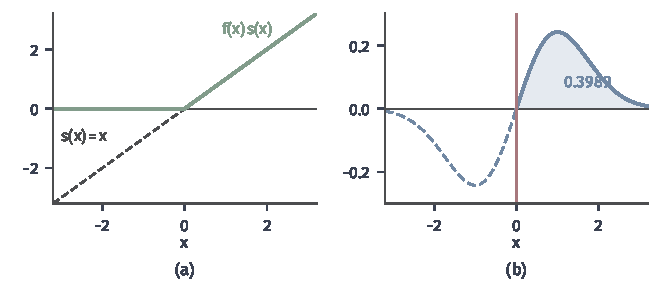
\includegraphics[width=112mm]{figures/07-probability/08-sampling-and-integration/matplotlib/pgrad-score-weights/figure.pdf}
  \caption{$X\sim\mathcal{N}(\theta,1)$在$\theta=0$处，$f(x)=\mathbf{1}_{\{x>0\}}$。(a)灰色虚线为得分$s(x)=x$，绿线为单样本估计的取值$f(x)s(x)$。(b)蓝线为$\partial_{\theta}p_{\theta}=p\,s$；红线$x=0$左侧$f=0$，这部分（虚线）不计入；右侧浅蓝面积为$\varphi(0)\approx0.3989$，等于$J'(0)$。}
  \label{fig:pgrad-score-weights}
\end{BookInlineFigure}

离散分布同样适用。$X\sim\operatorname{Bern}(\theta)$时，以计数测度为参考，$p_{\theta}(1)=\theta$，$p_{\theta}(0)=1-\theta$，得分为
\[
  s(1)=\frac{1}{\theta},\qquad s(0)=-\frac{1}{1-\theta},
\]
于是
\[
  \mathbb{E}[f(X)s(X)]=\theta\cdot\frac{f(1)}{\theta}-(1-\theta)\cdot\frac{f(0)}{1-\theta}=f(1)-f(0),
\]
正是图~\ref{fig:pgrad-bernoulli-threshold}中路径导数漏掉的那一项。

\paragraph{与重参数化在同一组样本上比较}

回到$X\sim\mathcal{N}(\mu,\sigma^{2})$、$f(x)=x^{2}$。由第~\ref{chap:information-geometry}章，两个得分分量是
\[
  s_{\mu}(x)=\frac{x-\mu}{\sigma^{2}}=\frac{\varepsilon}{\sigma},\qquad s_{\sigma}(x)=\frac{(x-\mu)^{2}-\sigma^{2}}{\sigma^{3}}=\frac{\varepsilon^{2}-1}{\sigma},
\]
其中$\varepsilon=(x-\mu)/\sigma$。用上一节同样的四个样本（$\mu=1$，$\sigma=0.5$），函数值是$f=1.3225,\ 0.2025,\ 1.9600,\ 0.6400$。$\mu$分量的单样本估计$f s_{\mu}$及其平均为
\[
  0.7935,\ -0.4455,\ 3.1360,\ -0.5120,\qquad\hat{g}_{\mu}=0.743,
\]
$\sigma$分量$f s_{\sigma}$为
\[
  -2.4069,\ 0.0851,\ -1.4112,\ -1.0752,\qquad\hat{g}_{\sigma}=-1.202 .
\]
真值是$(2,1)$，重参数化在同样的噪声上给出$(1.900,0.325)$。两种估计都无偏，但得分函数估计在这组样本上偏得更远，这不是偶然：第~\ref{sec:pgrad-variance}节会算出，在这个例子里得分函数估计的方差大得多。得分估计只利用“哪里的质量变多了”，不利用函数在样本附近怎样变化，丢掉了光滑性提供的信息。

\paragraph{支撑随参数移动}

定理~\ref{thm:pgrad-score}要求共同支撑。设$X\sim\operatorname{Unif}(0,\theta)$，$f(x)=x$，则$J(\theta)=\theta/2$，$J'(\theta)=\frac{1}{2}$。在支撑$(0,\theta)$内，$p_{\theta}(x)=1/\theta$，得分是常数$-1/\theta$。直接套用式~\eqref{eq:pgrad-score}，
\[
  \mathbb{E}_{\theta}[f(X)s_{\theta}(X)]=-\frac{1}{\theta}\mathbb{E}_{\theta}[X]=-\frac{1}{2},
\]
连符号都错了。

正确的计算要对积分上限求导。由含参积分的求导法则，
\[
  \frac{\mathrm{d}}{\mathrm{d}\theta}\int_{0}^{\theta}\frac{x}{\theta}\,\mathrm{d}x
  =\underbrace{\theta\cdot\frac{1}{\theta}}_{\text{边界}}+\int_{0}^{\theta}x\cdot\Bigl(-\frac{1}{\theta^{2}}\Bigr)\mathrm{d}x
  =1-\frac{1}{2}=\frac{1}{2}.
\]
第二项正是得分公式算出的$-\frac{1}{2}$，第一项$f(\theta)p_{\theta}(\theta^{-})=1$是新进入支撑的那一小段带来的贡献，得分只定义在旧支撑上，看不到它。第~\ref{chap:information-geometry}章用同一个均匀族说明了得分的期望在这里不为零，本例则显示加权以后漏掉的边界项可以比被计入的部分还大。

图~\ref{fig:pgrad-uniform-boundary}取$\theta=1$、$h=0.25$画出了两部分。旧支撑内$f p$从蓝线降到黄线，减少的面积是$0.1$；新增的一段$(1,1.25]$贡献$0.225$。净变化$0.125$等于$J(1.25)-J(1)$。除以$h$后两部分分别是$-0.4$与$0.9$，$h\to0$时趋于$-\frac{1}{2}$与$1$。

\begin{BookInlineFigure}
  \centering
  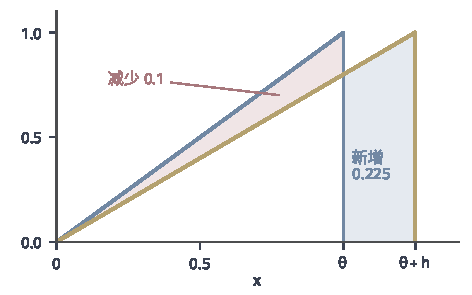
\includegraphics[width=80mm]{figures/07-probability/08-sampling-and-integration/matplotlib/pgrad-uniform-boundary/figure.pdf}
  \caption{$X\sim\operatorname{Unif}(0,\theta)$，$f(x)=x$。蓝线为$\theta=1$时的$f p_{\theta}$，黄线为$\theta+h=1.25$时的$f p_{\theta+h}$。浅红区域是旧支撑内减少的部分（面积$0.1$），得分公式只看到这一部分；浅蓝区域是新进入支撑的部分（面积$0.225$），得分公式漏掉了它。}
  \label{fig:pgrad-uniform-boundary}
\end{BookInlineFigure}

这个例子用重参数化反而没有困难：$X=\theta U$，$U\sim\operatorname{Unif}(0,1)$，路径导数$\frac{\mathrm{d}}{\mathrm{d}\theta}(\theta U)=U$，期望正是$\frac{1}{2}$。支撑的移动被样本点的移动自然地带了进去。两种方法的适用范围互补：重参数化怕函数沿路径跳跃，得分函数怕支撑随参数移动。

\subsection{未知归一化常数}
\label{sec:pgrad-score-unnormalized}

许多分布只能写到一个常数因子，例如未归一化密度取$\exp(-V_{\bm{\theta}}(x))$的形式，其中能量函数$V_{\bm{\theta}}$可以计算，而
\[
  Z_{\bm{\theta}}=\int\widetilde{p}_{\bm{\theta}}\,\mathrm{d}\nu
\]
在高维时无法直接求出。第~\ref{chap:sample-generation}章的Metropolis--Hastings采样正是为这种分布设计的：它只用到$\widetilde{p}_{\bm{\theta}}$的比值。现在要对归一化后的密度$p_{\bm{\theta}}$（即$\widetilde{p}_{\bm{\theta}}$除以$Z_{\bm{\theta}}$）下的期望求梯度，而$Z_{\bm{\theta}}$本身也随参数改变。

困难在于得分
\[
  \nabla_{\bm{\theta}}\ln p_{\bm{\theta}}=\nabla_{\bm{\theta}}\ln\widetilde{p}_{\bm{\theta}}-\nabla_{\bm{\theta}}\ln Z_{\bm{\theta}}
\]
含有$Z_{\bm{\theta}}$的导数。下面要说明，这个导数也可以写成目标分布下的期望，从而由目标样本计算。整个推导在同一个参考测度$\nu$与共同支撑$S=\{x:\widetilde{p}_{\bm{\theta}}(x)>0\}$上进行，并要求在以所论参数为中心的某个开球$U$内，每个$\bm{\theta}$都有$0<Z_{\bm{\theta}}<\infty$。需要两项交换条件：
\begin{enumerate}
  \item 归一化积分可以在积分号下求导：$\widetilde{p}_{\bm{\theta}}$在$S$上满足定理~\ref{thm:pgrad-exchange}的条件（$\mu=\nu$），于是$Z_{\bm{\theta}}$可微，梯度等于$\nabla_{\bm{\theta}}\widetilde{p}_{\bm{\theta}}$在$S$上的积分；
  \item 加权积分可以在积分号下求导：$f_{\bm{\theta}}\widetilde{p}_{\bm{\theta}}$也满足这些条件，于是加权积分
  \[
    N(\bm{\theta})=\int_{S}f_{\bm{\theta}}\widetilde{p}_{\bm{\theta}}\,\mathrm{d}\nu
  \]
  可微，梯度可在积分号下计算。
\end{enumerate}
两者缺一不可：$J=N/Z$，分子分母各自的导数都要能写成积分。

\subsubsection{得分的中心化}
\label{sec:pgrad-centering}

记未归一化密度的对数导数为
\[
  \bm{a}_{\bm{\theta}}(x)=\nabla_{\bm{\theta}}\ln\widetilde{p}_{\bm{\theta}}(x)=\frac{\nabla_{\bm{\theta}}\widetilde{p}_{\bm{\theta}}(x)}{\widetilde{p}_{\bm{\theta}}(x)},\qquad x\in S .
\]
它只用到$\widetilde{p}_{\bm{\theta}}$，可以在每个样本处计算。它和得分差多少？

\begin{lemma}[归一化常数的对数导数]
\label{lem:pgrad-logz}
在上述交换条件1下，$\bm{a}_{\bm{\theta}}(X)$在$P_{\bm{\theta}}$下可积，并且
\begin{equation}
  \nabla_{\bm{\theta}}\ln Z_{\bm{\theta}}=\mathbb{E}_{\bm{\theta}}[\bm{a}_{\bm{\theta}}(X)],
  \label{eq:pgrad-logz}
\end{equation}
从而得分是中心化的对数导数：
\begin{equation}
  \bm{s}_{\bm{\theta}}(x)=\bm{a}_{\bm{\theta}}(x)-\mathbb{E}_{\bm{\theta}}[\bm{a}_{\bm{\theta}}(X)].
  \label{eq:pgrad-centered-score}
\end{equation}
\end{lemma}

\begin{proof}
定理~\ref{thm:pgrad-exchange}的结论包含$\nabla_{\bm{\theta}}\widetilde{p}_{\bm{\theta}}$对$\nu$可积。由$\bm{a}_{\bm{\theta}}$的定义，在$S$上
\[
  \nabla_{\bm{\theta}}\widetilde{p}_{\bm{\theta}}=\widetilde{p}_{\bm{\theta}}\bm{a}_{\bm{\theta}}=Z_{\bm{\theta}}\,p_{\bm{\theta}}\bm{a}_{\bm{\theta}},
\]
所以
\[
  \mathbb{E}_{\bm{\theta}}\lVert\bm{a}_{\bm{\theta}}\rVert_{2}=\frac{1}{Z_{\bm{\theta}}}\int_{S}\lVert\nabla_{\bm{\theta}}\widetilde{p}_{\bm{\theta}}\rVert_{2}\,\mathrm{d}\nu<\infty .
\]
同一个关系与交换条件1给出
\[
  \nabla Z_{\bm{\theta}}=\int_{S}\widetilde{p}_{\bm{\theta}}\bm{a}_{\bm{\theta}}\,\mathrm{d}\nu=Z_{\bm{\theta}}\,\mathbb{E}_{\bm{\theta}}[\bm{a}_{\bm{\theta}}].
\]
因为$0<Z_{\bm{\theta}}<\infty$，两边除以$Z_{\bm{\theta}}$即得式~\eqref{eq:pgrad-logz}。最后，$\ln p_{\bm{\theta}}$与$\ln\widetilde{p}_{\bm{\theta}}$只差$\ln Z_{\bm{\theta}}$，对参数求梯度得到式~\eqref{eq:pgrad-centered-score}。
\end{proof}

这个结果的含义可以用质量的比喻说清楚。$\bm{a}_{\bm{\theta}}$记录的是未归一化质量在各位置的相对增长率，它完全可以处处为正：所有位置的质量都在增加。但概率的总量固定为$1$，归一化会把整体的增长除掉，只留下各位置相对于平均增长的差别。平均增长率按目标分布加权，就是$\mathbb{E}_{\bm{\theta}}[\bm{a}_{\bm{\theta}}]$，它等于$\ln Z_{\bm{\theta}}$的变化率。式~\eqref{eq:pgrad-centered-score}因此说：得分是相对增长率减去它的平均。中心化后的量期望为零，与第~\ref{chap:information-geometry}章得分期望为零的结论一致。

以三点分布为例。在$\{0,1,2\}$上取未归一化质量
\[
  \widetilde{p}_{\theta}(x)=h(x)\mathrm{e}^{\theta x},\qquad h=(1,2,1).
\]
此时
\[
  a_{\theta}(x)=x,\qquad Z_{\theta}=1+2\mathrm{e}^{\theta}+\mathrm{e}^{2\theta}=(1+\mathrm{e}^{\theta})^{2}.
\]
归一化后$p_{\theta}$是二项分布$\operatorname{Bin}(2,q)$，其中$q=\mathrm{e}^{\theta}/(1+\mathrm{e}^{\theta})$。直接求导得到
\[
  \frac{\mathrm{d}}{\mathrm{d}\theta}\ln Z_{\theta}=\frac{2\mathrm{e}^{\theta}}{1+\mathrm{e}^{\theta}}=2q,
\]
正是$\mathbb{E}_{\theta}[X]$，与式~\eqref{eq:pgrad-logz}一致。在$\theta=0$处，分布是$(\frac{1}{4},\frac{1}{2},\frac{1}{4})$，$a$的期望为$1$，得分是$s_{0}(x)=x-1$。

图~\ref{fig:pgrad-unnormalized}画出了这个过程。$\theta$由$0$增至$0.5$时，未归一化的三根柱子没有一根变矮；归一化以后，$x=0$处的概率从$0.25$降到约$0.14$，$x=2$处从$0.25$升到约$0.39$。$a(x)=x$全非负，减去平均$1$后才得到有正有负的得分。指数族是这个例子的一般形式：$\bm{a}_{\bm{\theta}}=\bm{T}(x)$，式~\eqref{eq:pgrad-centered-score}就是第~\ref{chap:information-geometry}章的$\bm{T}-\mathbb{E}_{\bm{\theta}}[\bm{T}]$。

\begin{BookInlineFigure}
  \centering
  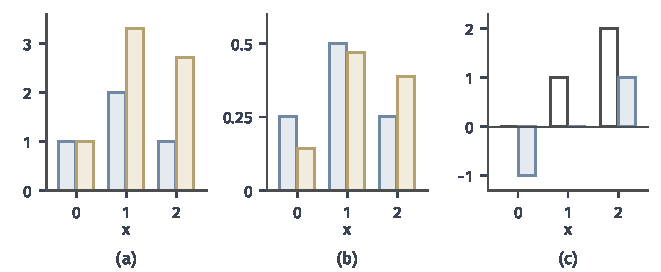
\includegraphics[width=112mm]{figures/07-probability/08-sampling-and-integration/matplotlib/pgrad-unnormalized/figure.pdf}
  \caption{$\{0,1,2\}$上的$\widetilde{p}_{\theta}(x)=h(x)\mathrm{e}^{\theta x}$，$h=(1,2,1)$。(a)未归一化质量，蓝色为$\theta=0$（总量$Z=4$），黄色为$\theta=0.5$（总量约$7.02$）；(b)归一化后的概率，质量从$x=0$移向$x=2$；(c)空心柱为$a(x)=x$，蓝色柱为$\theta=0$处的得分$s(x)=x-1$。}
  \label{fig:pgrad-unnormalized}
\end{BookInlineFigure}

\subsubsection{协方差形式}
\label{sec:pgrad-covariance}

有了中心化的得分，可以把式~\eqref{eq:pgrad-score}改写成不含$Z_{\bm{\theta}}$的形式。对标量函数$f$与向量函数$\bm{a}$，记
\[
  \operatorname{Cov}_{\bm{\theta}}(f,\bm{a})=\mathbb{E}_{\bm{\theta}}[f\bm{a}]-\mathbb{E}_{\bm{\theta}}[f]\,\mathbb{E}_{\bm{\theta}}[\bm{a}]\in\mathbb{R}^{k},
\]
它的第$j$个分量是$f$与$a_{j}$的协方差。这个定义只用到$f$、$\bm{a}$与$f\bm{a}$的可积性，不要求二阶矩。

\begin{theorem}[协方差形式的梯度]
\label{thm:pgrad-covariance}
在交换条件1与条件2下，若$f_{\bm{\theta}}$、$\nabla_{\bm{\theta}}f_{\bm{\theta}}$与$f_{\bm{\theta}}\bm{a}_{\bm{\theta}}$在$P_{\bm{\theta}}$下可积，则
\begin{equation}
  \nabla J(\bm{\theta})=\mathbb{E}_{\bm{\theta}}\bigl[\nabla_{\bm{\theta}}f_{\bm{\theta}}(X)\bigr]+\operatorname{Cov}_{\bm{\theta}}\bigl(f_{\bm{\theta}}(X),\bm{a}_{\bm{\theta}}(X)\bigr).
  \label{eq:pgrad-covariance}
\end{equation}
\end{theorem}

\begin{proof}
$J$是交换条件2中的加权积分$N$与$Z_{\bm{\theta}}$之比。由交换条件2，
\[
  \nabla N=\int_{S}\bigl(\nabla_{\bm{\theta}}f_{\bm{\theta}}+f_{\bm{\theta}}\bm{a}_{\bm{\theta}}\bigr)\widetilde{p}_{\bm{\theta}}\,\mathrm{d}\nu=Z_{\bm{\theta}}\,\mathbb{E}_{\bm{\theta}}\bigl[\nabla_{\bm{\theta}}f_{\bm{\theta}}+f_{\bm{\theta}}\bm{a}_{\bm{\theta}}\bigr],
\]
其中拆成两个期望用到了所设的可积性。由交换条件1与引理~\ref{lem:pgrad-logz}的证明，$\nabla Z_{\bm{\theta}}$等于$Z_{\bm{\theta}}\mathbb{E}_{\bm{\theta}}[\bm{a}_{\bm{\theta}}]$。商的求导法则给出
\[
  \nabla J=\frac{\nabla N}{Z_{\bm{\theta}}}-\frac{N}{Z_{\bm{\theta}}}\cdot\frac{\nabla Z_{\bm{\theta}}}{Z_{\bm{\theta}}}
  =\mathbb{E}_{\bm{\theta}}\bigl[\nabla_{\bm{\theta}}f_{\bm{\theta}}+f_{\bm{\theta}}\bm{a}_{\bm{\theta}}\bigr]-\mathbb{E}_{\bm{\theta}}[f_{\bm{\theta}}]\,\mathbb{E}_{\bm{\theta}}[\bm{a}_{\bm{\theta}}],
\]
整理即得式~\eqref{eq:pgrad-covariance}。
\end{proof}

逐个分量看，第$j$个分量的第二项是$\operatorname{Cov}_{\bm{\theta}}(f,a_{j})$。沿第$j$个参数方向，未归一化质量在$x$处按相对速率$a_{j}(x)$增长。若增长得快的地方恰好是$f$大的地方，协方差为正，期望上升；若两者无关，协方差为零，质量的增长只是整体放大，归一化后什么也没有改变。给$a_{j}$加上任何常数（各处等速增长）都不改变协方差。$\ln Z_{\bm{\theta}}$的导数正是以这种方式计入的：协方差中减去的$\mathbb{E}[f]\mathbb{E}[a_{j}]$就是那一项，而计算它只需要目标样本，不需要知道$Z_{\bm{\theta}}$。

在三点分布的例子中取$f(x)=x^{2}$，与参数无关。在$\theta=0$处，
\[
  \mathbb{E}_{0}[f]=\tfrac{0+2+4}{4}=1.5,\quad\mathbb{E}_{0}[a]=1,\quad\mathbb{E}_{0}[fa]=\mathbb{E}_{0}[X^{3}]=\tfrac{0+2+8}{4}=2.5,
\]
于是$J'(0)=\operatorname{Cov}_{0}(X^{2},X)=2.5-1.5=1$。用闭式核对：$X\sim\operatorname{Bin}(2,q)$时$J=\mathbb{E}[X^{2}]=2q+2q^{2}$，而$\mathrm{d}q/\mathrm{d}\theta=q(1-q)$，所以
\[
  J'(\theta)=(2+4q)\,q(1-q),
\]
在$q=\frac{1}{2}$处等于$4\cdot\frac{1}{4}=1$，两种算法一致。

\subsubsection{样本估计}
\label{sec:pgrad-cov-sample}

式~\eqref{eq:pgrad-covariance}中的期望与协方差都要用目标样本估计。设$X_{1},\dots,X_{n}$（$n\geq2$）独立同分布于$P_{\bm{\theta}}$，记$F_{i}=f_{\bm{\theta}}(X_{i})$，$\bm{A}_{i}=\bm{a}_{\bm{\theta}}(X_{i})$，$\bar{F}$与$\bar{\bm{A}}$为样本平均。以样本平均作中心的协方差估计取分母$n-1$：
\begin{equation}
  \hat{\bm{C}}_{n}=\frac{1}{n-1}\sum_{i=1}^{n}(F_{i}-\bar{F})(\bm{A}_{i}-\bar{\bm{A}}).
  \label{eq:pgrad-cov-estimator}
\end{equation}
梯度的估计是$\frac{1}{n}\sum_{i}\nabla_{\bm{\theta}}f_{\bm{\theta}}(X_{i})+\hat{\bm{C}}_{n}$。

为什么是$n-1$？展开乘积，
\[
  \sum_{i=1}^{n}(F_{i}-\bar{F})(\bm{A}_{i}-\bar{\bm{A}})=\sum_{i=1}^{n}F_{i}\bm{A}_{i}-n\bar{F}\bar{\bm{A}} .
\]
第一项的期望是$n\,\mathbb{E}[f\bm{a}]$。第二项里
\[
  \bar{F}\bar{\bm{A}}=\frac{1}{n^{2}}\sum_{i=1}^{n}\sum_{j=1}^{n}F_{i}\bm{A}_{j},
\]
其中$n$个$i=j$的项期望为$\mathbb{E}[f\bm{a}]$，其余$n(n-1)$项由独立性期望为$\mathbb{E}[f]\mathbb{E}[\bm{a}]$，所以
\[
  \mathbb{E}\bigl[n\bar{F}\bar{\bm{A}}\bigr]=\mathbb{E}[f\bm{a}]+(n-1)\,\mathbb{E}[f]\,\mathbb{E}[\bm{a}].
\]
两式相减，
\[
  \mathbb{E}\Bigl[\sum_{i=1}^{n}(F_{i}-\bar{F})(\bm{A}_{i}-\bar{\bm{A}})\Bigr]=(n-1)\operatorname{Cov}_{\bm{\theta}}(f,\bm{a}).
\]
用样本平均作中心时，每个样本都参与了它自己的中心，这使乘积系统地偏小，损失恰好是一个样本的份额。除以$n-1$得到无偏估计；除以$n$则期望为$\frac{n-1}{n}\operatorname{Cov}_{\bm{\theta}}(f,\bm{a})$，小样本时偏差明显。推导只用到独立同分布和$f$、$\bm{a}$、$f\bm{a}$的可积性。

用三点分布在$\theta=0$处手算一次。由逆变换，累积概率的分点是$0.25$与$0.75$，均匀数$u=0.37,0.80,0.15,0.62$给出
\[
  X=1,\ 2,\ 0,\ 1,\qquad F=1,\ 4,\ 0,\ 1,\qquad A=1,\ 2,\ 0,\ 1 .
\]
样本平均为$\bar{F}=1.5$、$\bar{A}=1$，中心化后的乘积依次是
\[
  (-0.5)\cdot0,\quad2.5\cdot1,\quad(-1.5)\cdot(-1),\quad(-0.5)\cdot0,
\]
和为$4$。除以$n-1=3$得$\hat{C}_{4}=1.333$，除以$n=4$得$1$。真值是$1$；这一组样本恰好让有偏的版本更接近真值，但平均而言它偏小$25\%$。图~\ref{fig:pgrad-cov-bias}用大量重复显示了两种分母的平均行为。

\begin{BookInlineFigure}
  \centering
  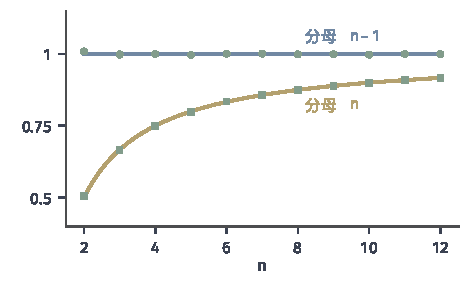
\includegraphics[width=80mm]{figures/07-probability/08-sampling-and-integration/matplotlib/pgrad-cov-bias/figure.pdf}
  \caption{三点分布$p_{0}=(\frac{1}{4},\frac{1}{2},\frac{1}{4})$上$\operatorname{Cov}(X^{2},X)=1$的两种样本估计。蓝线与绿色圆点：分母$n-1$，期望恒为$1$；黄线与绿色方块：分母$n$，期望$(n-1)/n$。线为精确期望，点为每个$n$重复$40000$次（固定种子）的平均。}
  \label{fig:pgrad-cov-bias}
\end{BookInlineFigure}

这个无偏保证依赖独立同分布。未归一化目标的样本通常来自MCMC，链上的样本相关，而且从一般初值出发时各时刻的分布还不是$P_{\bm{\theta}}$。这时推导中“$i\neq j$的项期望为$\mathbb{E}[f]\mathbb{E}[\bm{a}]$”不再成立，$n-1$分母不再修正什么，有限样本偏差由链的初值与相关性决定，要按第~\ref{sec:pgrad-approx}节与第~\ref{chap:monte-carlo-integration-error}章检查。若改用自归一化重要性采样的加权样本，加权协方差是两个随机量之比，有限样本下一般有偏，要按第~\ref{chap:variance-reduction}章对比值估计的分析检查。无偏只是一阶的性质，估计的二阶矩是否有限、波动有多大，是下一节的问题。

\section{梯度估计的方差控制}
\label{sec:pgrad-variance}

前三节得到了同一个梯度的几种表示。以$X\sim\mathcal{N}(\theta,1)$、$f(x)=x^{2}$为例，路径导数$2X$与得分估计$X^{2}(X-\theta)$的期望都是$2\theta$，它们是同一个向量期望的不同计算公式。第~\ref{chap:variance-reduction}章的观点在这里完全适用：期望相同的计算公式之间可以比较方差，也可以用控制变量和条件期望改造公式，只要改造不改变期望。

\paragraph{比较的对象}

梯度估计是$\mathbb{R}^{k}$值的，单样本$\bm{G}$的波动由协方差矩阵$\bm{\Sigma}_{\bm{G}}$描述。比较两个估计时，可以逐分量比较方差$(\bm{\Sigma}_{\bm{G}})_{j,j}$，也可以沿指定方向$\bm{u}$比较
\[
  \operatorname{Var}\bigl(\langle\bm{u},\bm{G}\rangle\bigr)=\bm{u}^{\top}\bm{\Sigma}_{\bm{G}}\bm{u},
\]
或比较式~\eqref{eq:pgrad-direct-mse}中的迹。不同分量的精度可以相差很大，第~\ref{sec:pgrad-reparam}节的高斯例子里，$\mu$分量与$\sigma$分量的单样本方差分别是$1$和$6$。这些比较都以$\mathbb{E}\lVert\bm{G}\rVert_{2}^{2}<\infty$为前提，要对每个用到的分量分别核对。

先把高斯例子的两个方差算出来。重参数化的单样本$2X$方差为$4$。得分估计是$X^{2}\varepsilon$，其中$\varepsilon=X-\theta$。求它的二阶矩要展开$(\theta+\varepsilon)^{4}\varepsilon^{2}$，所用的标准正态矩是
\[
  \mathbb{E}[\varepsilon^{2}]=1,\qquad\mathbb{E}[\varepsilon^{4}]=3,\qquad\mathbb{E}[\varepsilon^{6}]=15,
\]
奇数阶矩为零。只保留偶数次项，得到
\[
  \mathbb{E}\bigl[(\theta+\varepsilon)^{4}\varepsilon^{2}\bigr]=\theta^{4}+6\theta^{2}\cdot3+15=\theta^{4}+18\theta^{2}+15 .
\]
减去均值的平方$4\theta^{2}$，方差为$\theta^{4}+14\theta^{2}+15$。在$\theta=1$处是$30$，约为重参数化的$7.5$倍：要达到同样的精度，得分估计需要约$7.5$倍的样本。

\paragraph{得分作为控制变量}

得分估计的方差大，一个原因可以直接看出。由第~\ref{chap:information-geometry}章，正则族的得分期望为零。于是对任意常数$b$，
\[
  \mathbb{E}\bigl[(f(X)-b)\,s(X)\bigr]=\mathbb{E}[f(X)s(X)]-b\,\mathbb{E}[s(X)]=\mathbb{E}[f(X)s(X)],
\]
期望不变。项$b\,s(X)$是纯粹的噪声：它的平均为零，却随样本上下波动。在高斯例子里$f=X^{2}$总是正的，$f s$的波动有相当一部分来自$f$的平均水平乘上$s$的符号；减去一个接近$f$平均水平的$b$，就把这部分去掉了。这个常数$b$称为\term{基线}（baseline）。

这正是第~\ref{chap:variance-reduction}章的控制变量：辅助函数$h=s_{j}$的期望已知为零，系数为$b$。各分量可以用不同的基线$b_{j}$。若$\mathbb{E}[f^{2}s_{j}^{2}]<\infty$且$0<\mathbb{E}[s_{j}^{2}]<\infty$，第$j$个分量的方差是
\[
  V_{j}(b_{j})=\mathbb{E}\bigl[(f-b_{j})^{2}s_{j}^{2}\bigr]-\bigl(\mathbb{E}[f s_{j}]\bigr)^{2},
\]
它是$b_{j}$的二次函数。对$b_{j}$求导并令其为零，$-2\mathbb{E}[(f-b_{j})s_{j}^{2}]=0$，得到最优基线
\begin{equation}
  b_{j}^{*}=\frac{\mathbb{E}\bigl[f(X)\,s_{j}(X)^{2}\bigr]}{\mathbb{E}\bigl[s_{j}(X)^{2}\bigr]}.
  \label{eq:pgrad-optimal-baseline}
\end{equation}
它是按$s_{j}^{2}$加权的$f$的平均：得分大的样本对估计影响大，基线应当贴近这些样本上的函数值。由于$\mathbb{E}[s_{j}]=0$，它与控制变量的最优系数$\operatorname{Cov}(fs_{j},s_{j})/\operatorname{Var}(s_{j})$一致。

在高斯例子中，同样只保留偶数次项，
\[
  \mathbb{E}[f s^{2}]=\mathbb{E}\bigl[(\theta+\varepsilon)^{2}\varepsilon^{2}\bigr]=\theta^{2}+3,\qquad\mathbb{E}[s^{2}]=1,
\]
所以$b^{*}=\theta^{2}+3$。在$\theta=1$处，前面算出的$\mathbb{E}[f^{2}s^{2}]$等于$34$，方差作为$b$的函数是
\[
  V(b)=34-8b+b^{2}-4=b^{2}-8b+30 .
\]
三个基线的结果是
\[
  V(0)=30,\qquad V(J(1))=V(2)=18,\qquad V(b^{*})=V(4)=14 .
\]
用$J(\theta)=\mathbb{E}[f]$作基线是常见的简便选择，这里它把方差从$30$降到$18$；最优基线降到$14$。图~\ref{fig:pgrad-baseline-var}画出了这条抛物线。即使用最优基线，得分估计仍不如重参数化的$4$：常数基线只能去掉与$s$成比例的那部分噪声。

\begin{BookInlineFigure}
  \centering
  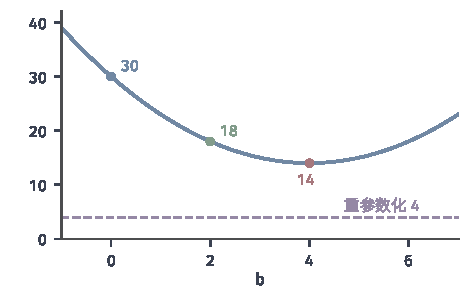
\includegraphics[width=80mm]{figures/07-probability/08-sampling-and-integration/matplotlib/pgrad-baseline-var/figure.pdf}
  \caption{$X\sim\mathcal{N}(1,1)$，$f(x)=x^{2}$。单样本估计$(f(X)-b)(X-1)$的方差$V(b)=b^{2}-8b+30$（蓝线）。蓝点为无基线$b=0$，绿点为$b=J(1)=2$，红点为最优基线$b^{*}=4$；紫色虚线为重参数化估计$2X$的方差$4$。}
  \label{fig:pgrad-baseline-var}
\end{BookInlineFigure}

\paragraph{基线所用的数据}

最优基线含有未知的期望，实际中要用样本估计。这时必须注意：$\mathbb{E}[b\,s(X)]=0$的推导要求$b$是常数，或者至少与$X$独立。若$b$由与当前样本独立的数据算出（例如先前单独抽取的一批试运行样本），则在给定这批数据的条件下$b$是常数，估计条件无偏，因而无偏。若$b$用到了当前样本本身，就要重新检查。

最自然的错误是用全部样本的平均$\bar{F}=\frac{1}{n}\sum_{j}f(X_{j})$作基线。对第$i$项，
\[
  \mathbb{E}\bigl[\bar{F}s(X_{i})\bigr]=\frac{1}{n}\mathbb{E}\bigl[f(X_{i})s(X_{i})\bigr]+\frac{1}{n}\sum_{j\neq i}\mathbb{E}[f(X_{j})]\,\mathbb{E}[s(X_{i})]=\frac{1}{n}J'(\theta),
\]
因为$\bar{F}$里含有$f(X_{i})$，它与$s(X_{i})$相关。于是
\[
  \mathbb{E}\bigl[(f(X_{i})-\bar{F})\,s(X_{i})\bigr]=\Bigl(1-\frac{1}{n}\Bigr)J'(\theta),
\]
估计系统地偏小。这和第~\ref{sec:pgrad-cov-sample}节样本协方差的偏差是同一个来源。

修正的办法是让每个样本的基线不含它自己：用其余$n-1$个样本的平均
\[
  b_{i}=\bar{F}_{-i}=\frac{1}{n-1}\sum_{j\neq i}f(X_{j}),
\]
称为\term{留一基线}（leave-one-out baseline）。$b_{i}$与$X_{i}$独立，所以$\mathbb{E}[(f(X_{i})-b_{i})s(X_{i})]=J'(\theta)$，估计无偏。由$\bar{F}_{-i}=(n\bar{F}-f(X_{i}))/(n-1)$，直接算出
\[
  f(X_{i})-\bar{F}_{-i}=\frac{n}{n-1}\bigl(f(X_{i})-\bar{F}\bigr),
\]
所以留一基线的估计恰好是全平均基线估计乘以$\frac{n}{n-1}$，与样本协方差的$n-1$分母是同一个修正。

下面用固定噪声手算。$\theta=1$，$\varepsilon=0.3,-1.1,0.8,-0.4$，样本$X=1.3,\,-0.1,\,1.8,\,0.6$，函数值与得分为
\[
  f=1.69,\ 0.01,\ 3.24,\ 0.36,\qquad s=0.3,\ -1.1,\ 0.8,\ -0.4 .
\]
不用基线时，$f s=0.507,\ -0.011,\ 2.592,\ -0.144$，平均为$0.736$。全平均为$\bar{F}=1.325$，四个留一基线是
\[
  b_{i}=1.2033,\ 1.7633,\ 0.6867,\ 1.6467,
\]
对应的$(f-b_{i})s=0.1460,\ 1.9287,\ 2.0427,\ 0.5147$，平均为$1.158$。用全平均作基线得到$0.8685$，正好是$1.158\times\frac{3}{4}$。真值是$2$。四个样本太少，三者都偏离真值，但只有前两种在平均意义下是无偏的。图~\ref{fig:pgrad-loo-baseline}用大量重复验证了全平均基线的偏差因子$\frac{n-1}{n}$。

\begin{BookInlineFigure}
  \centering
  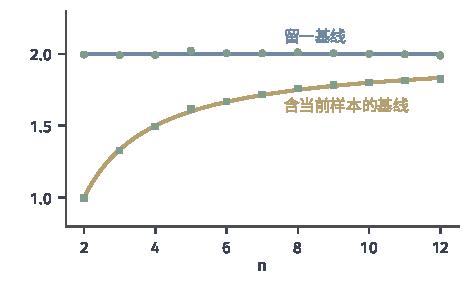
\includegraphics[width=80mm]{figures/07-probability/08-sampling-and-integration/matplotlib/pgrad-loo-baseline/figure.pdf}
  \caption{$X\sim\mathcal{N}(1,1)$，$f(x)=x^{2}$，真值$J'(1)=2$。蓝线与绿色圆点：留一基线估计的期望（恒为$2$）；黄线与绿色方块：以含当前样本的全平均作基线的估计，期望为$2(n-1)/n$。线为精确值，点为每个$n$重复$40000$次（固定种子）的平均。}
  \label{fig:pgrad-loo-baseline}
\end{BookInlineFigure}

教训是：依赖当前样本的修正不能默认无偏。留一基线之所以无偏，是因为每一项的基线与该项的得分独立；任意用当前样本拟合出来的修正项都要像上面这样逐项核对期望。

\paragraph{条件期望}

第~\ref{chap:variance-reduction}章的另一种方法是把能解析算出的随机性先积掉。设$X=(X_{1},X_{2})$，$X_{1}\sim\mathcal{N}(\theta,1)$与$X_{2}\sim\mathcal{N}(0,1)$独立，$f(x)=x_{1}^{2}+x_{2}^{2}$。参数只在$X_{1}$的分布里，得分是$s=X_{1}-\theta$，单样本得分估计为$(X_{1}^{2}+X_{2}^{2})(X_{1}-\theta)$。其中$X_{2}^{2}$与参数无关，却乘在$s$上增加波动。给定$X_{1}$对$X_{2}$取条件期望，$\mathbb{E}[X_{2}^{2}]=1$，得到改造后的估计
\[
  \mathbb{E}\bigl[(X_{1}^{2}+X_{2}^{2})s\mid X_{1}\bigr]=(X_{1}^{2}+1)(X_{1}-\theta).
\]

期望不变。记原估计为$G$，由全方差公式，方差减少的量是
\[
  \mathbb{E}\bigl[\operatorname{Var}(G\mid X_{1})\bigr]=\mathbb{E}[s^{2}]\operatorname{Var}(X_{2}^{2})=1\cdot2=2 .
\]
在$\theta=1$处可以直接核对。记$f_{1}=X_{1}^{2}$，前面已经算出$f_{1}^{2}s^{2}$与$f_{1}s^{2}$的期望分别是$34$与$4$；又$X_{2}^{2}$与$X_{2}^{4}$的期望分别是$1$与$3$。展开平方后逐项取期望，两个估计的二阶矩分别是
\[
  34+2\cdot4\cdot1+3\cdot1=45,\qquad34+2\cdot4+1=43,
\]
减去$J'(1)^{2}=4$后方差为$41$与$39$。条件化与基线可以叠加使用：在$(X_{1}^{2}+1)s$上再减去基线，就回到了一维问题的抛物线。

\paragraph{两种表示哪个更好}

在高斯二次函数的例子里，重参数化全面占优。从图~\ref{fig:pgrad-variance-compare}(a)可以看到，在$\theta\in[-2,2]$上它的方差恒为$4$，而得分估计即使配上最优基线也在$6$以上，并随$\lvert\theta\rvert$增长。但这不是普遍规律。路径导数用到$f$对$x$的导数，$f$变化剧烈时这个导数会放大波动；得分估计只用到$f$的值。

取$f(x)=\sin(\omega x)$，$X\sim\mathcal{N}(\theta,1)$。路径导数是$\omega\cos(\omega X)$，幅度随$\omega$增大；得分估计是$\sin(\omega X)(X-\theta)$，$\lvert\sin\rvert\leq1$限制了它。计算方差要用到两个高斯积分：
\[
  \mathbb{E}[\cos(cX)]=\mathrm{e}^{-c^{2}/2}\cos(c\theta),\qquad\mathbb{E}\bigl[\varepsilon^{2}\mathrm{e}^{\mathrm{i}c\varepsilon}\bigr]=(1-c^{2})\mathrm{e}^{-c^{2}/2},
\]
后者是标准正态特征函数$\mathrm{e}^{-c^{2}/2}$的二阶导数取负号。再用倍角公式把$\cos^{2}(\omega X)$与$\sin^{2}(\omega X)$写成$\cos(2\omega X)$的线性函数，在$\theta=0$处两者的方差为
\begin{align}
  \operatorname{Var}_{\mathrm{rep}}&=\frac{\omega^{2}}{2}\bigl(1+\mathrm{e}^{-2\omega^{2}}\bigr)-\omega^{2}\mathrm{e}^{-\omega^{2}},\label{eq:pgrad-sin-rep}\\
  \operatorname{Var}_{\mathrm{sf}}&=\frac{1}{2}\bigl(1-(1-4\omega^{2})\mathrm{e}^{-2\omega^{2}}\bigr)-\omega^{2}\mathrm{e}^{-\omega^{2}}.\label{eq:pgrad-sin-sf}
\end{align}

两式中减去的$\omega^{2}\mathrm{e}^{-\omega^{2}}$是$J'(0)^{2}$。$\omega\to\infty$时式~\eqref{eq:pgrad-sin-rep}像$\omega^{2}/2$那样增长，式~\eqref{eq:pgrad-sin-sf}趋于$\frac{1}{2}$。图~\ref{fig:pgrad-variance-compare}(b)显示两条曲线在$\omega\approx1.12$处相交，此后得分估计更好。

\begin{BookInlineFigure}
  \centering
  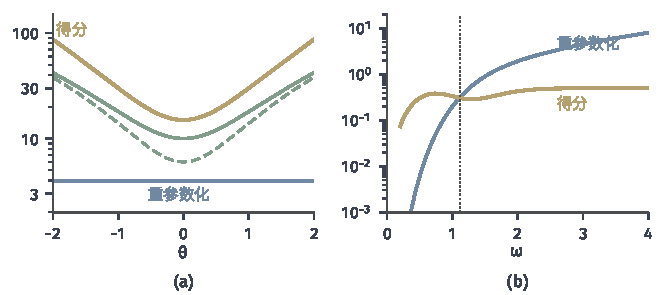
\includegraphics[width=112mm]{figures/07-probability/08-sampling-and-integration/matplotlib/pgrad-variance-compare/figure.pdf}
  \caption{$X\sim\mathcal{N}(\theta,1)$时单样本梯度估计的方差（对数纵轴）。(a)$f(x)=x^{2}$：蓝线为重参数化（恒为$4$），黄线为得分估计$\theta^{4}+14\theta^{2}+15$，绿实线为以$J(\theta)$为基线的得分估计$8\theta^{2}+10$，绿虚线为最优基线下的$8\theta^{2}+6$。(b)$f(x)=\sin(\omega x)$，$\theta=0$：蓝线为式~\eqref{eq:pgrad-sin-rep}，黄线为式~\eqref{eq:pgrad-sin-sf}，点线标出交点$\omega\approx1.12$。}
  \label{fig:pgrad-variance-compare}
\end{BookInlineFigure}

所以选择表示时不能预设哪一种更好。可用性由前几节的条件决定：函数沿路径是否受Lipschitz控制，得分能否计算，支撑是否随参数移动。在都可用的情形下，比较的是同一梯度任务下的方差与单样本成本；把这一比较放进整体预算，是下一章的内容。

\section{近似采样下的梯度}
\label{sec:pgrad-approx}

前面的无偏结论都假设样本精确服从$P_{\bm{\theta}}$。实际上，样本常常来自近似的生成器，或来自运行了有限步的Markov链。梯度公式本身是对的，用的样本却不对，结果算的是什么？

\paragraph{三个量}

设梯度公式$\bm{G}=\bm{\phi}_{\bm{\theta}}(X)$在目标下正确，即它在$X\sim P_{\bm{\theta}}$时的期望等于$\nabla J(\bm{\theta})$，而实际样本服从另一个分布$\widetilde{P}_{\bm{\theta}}$。要区分三个量：目标期望的梯度$\nabla J(\bm{\theta})$；公式在实际抽样规律下的均值
\[
  \bar{\bm{g}}(\bm{\theta})=\mathbb{E}_{\widetilde{P}_{\bm{\theta}}}[\bm{\phi}_{\bm{\theta}}(X)];
\]
以及$n$个样本平均$\hat{\bm{g}}_{n}$的有限样本波动。估计误差相应地分成两部分，
\begin{equation}
  \hat{\bm{g}}_{n}-\nabla J(\bm{\theta})=\underbrace{\bigl(\bar{\bm{g}}(\bm{\theta})-\nabla J(\bm{\theta})\bigr)}_{\text{采样偏差}}+\underbrace{\bigl(\hat{\bm{g}}_{n}-\bar{\bm{g}}(\bm{\theta})\bigr)}_{\text{有限样本波动}}.
  \label{eq:pgrad-error-split}
\end{equation}
这和第~\ref{chap:monte-carlo-integration-error}章对积分误差的分解完全相同，因为梯度估计本来就是一个积分估计。

第一部分与样本数无关，增加同一近似方法的样本数不能消除它。若$\bm{\phi}_{\bm{\theta}}$的分量有界，它可以用$\widetilde{P}_{\bm{\theta}}$与$P_{\bm{\theta}}$的总变差距离控制：对取值于$[m_{j},M_{j}]$的分量，偏差的绝对值不超过$(M_{j}-m_{j})\,d_{\mathrm{TV}}(\widetilde{P}_{\bm{\theta}},P_{\bm{\theta}})$。但梯度公式往往无界，例如得分估计里的$f\cdot s$，这时还需要尾部或矩的控制，分布在总变差下接近并不保证期望接近。第二部分取决于样本之间的关系：独立样本时它的方差是单样本方差除以$n$；样本是链上的连续状态时，要用第~\ref{chap:monte-carlo-integration-error}章的长期方差代替单样本方差，相关性可以使误差成倍增大。

\paragraph{一个可以算到底的链}

取目标$\mathcal{N}(\theta,1)$，$f(x)=x^{2}$，$J'(\theta)=2\theta$。用如下的链近似采样：
\[
  X^{(t+1)}=\rho X^{(t)}+(1-\rho)\theta+\sqrt{1-\rho^{2}}\,\varepsilon_{t},\qquad X^{(0)}=0,
\]
$\varepsilon_{t}$独立同分布于$\mathcal{N}(0,1)$，$0<\rho<1$。若$X^{(t)}\sim\mathcal{N}(\theta,1)$，则$X^{(t+1)}$的均值为$\rho\theta+(1-\rho)\theta=\theta$，方差为$\rho^{2}+1-\rho^{2}=1$，所以目标是这条链的不变分布。从$X^{(0)}=0$出发，均值与方差满足
\[
  m_{t+1}=\rho m_{t}+(1-\rho)\theta,\qquad v_{t+1}=\rho^{2}v_{t}+1-\rho^{2},
\]
解出第$K$步$X^{(K)}\sim\mathcal{N}(m_{K},v_{K})$，其中
\begin{equation}
  m_{K}=\theta(1-\rho^{K}),\qquad v_{K}=1-\rho^{2K}.
  \label{eq:pgrad-ar-law}
\end{equation}

把目标下正确的两个公式用在$X^{(K)}$上。重参数化公式$2X$的均值是$2m_{K}=2\theta(1-\rho^{K})$；得分公式$X^{2}(X-\theta)$的均值是
\[
  \mathbb{E}\bigl[(X^{(K)})^{3}\bigr]-\theta\,\mathbb{E}\bigl[(X^{(K)})^{2}\bigr]=m_{K}^{3}+3m_{K}v_{K}-\theta(m_{K}^{2}+v_{K}).
\]
取$\theta=1$、$\rho=0.8$、$K=5$，$\rho^{5}=0.32768$，于是$m_{5}=0.6723$，$v_{5}=0.8926$。两个公式的均值分别为
\[
  2m_{5}=1.345,\qquad m_{5}^{3}+3m_{5}v_{5}-(m_{5}^{2}+v_{5})=0.760,
\]
目标是$2$。同一组近似样本上，两个在目标下都无偏的公式偏差不同，偏差的大小取决于公式本身。

\paragraph{对有限步程序求导}

另一种做法是把整个采样程序当成生成映射，对它做重参数化。展开递推，$X^{(K)}$是$\theta$的仿射函数加上与$\theta$无关的噪声，$\partial X^{(K)}/\partial\theta=1-\rho^{K}$，路径导数为$2X^{(K)}(1-\rho^{K})$。这里每一步都合法：噪声分布固定，函数光滑，交换条件也容易验证。它的期望是程序所定义的期望
\[
  J_{K}(\theta)=\mathbb{E}\bigl[(X^{(K)})^{2}\bigr]=\theta^{2}(1-\rho^{K})^{2}+1-\rho^{2K}
\]
的导数$J_{K}'(\theta)=2\theta(1-\rho^{K})^{2}$，在上面的参数下等于$0.904$，而不是$J'(1)=2$。

也就是说，对有限步采样程序求导并交换积分，得到的是程序期望$J_{K}$的导数；它是否等于目标期望$J$的导数，是另一个需要证明的命题。本例中$J_{K}$对$\theta$的依赖还包含初值$X^{(0)}=0$不随$\theta$移动这一人为因素，所以$J_{K}'$比两个“目标公式”偏得更多。图~\ref{fig:pgrad-chain-bias}画出了三个量随步数$K$的变化，图~\ref{fig:pgrad-error-split}在$K=5$处把式~\eqref{eq:pgrad-error-split}的两部分和程序导数放在一条数轴上比较。

\begin{BookInlineFigure}
  \centering
  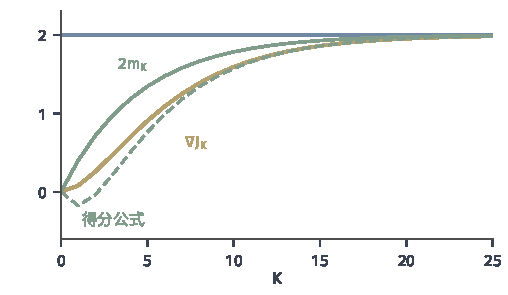
\includegraphics[width=86mm]{figures/07-probability/08-sampling-and-integration/matplotlib/pgrad-chain-bias/figure.pdf}
  \caption{目标$\mathcal{N}(1,1)$、$f(x)=x^{2}$，样本取自从$0$出发、$\rho=0.8$的链的第$K$步。蓝线为目标梯度$2$；绿实线为重参数化公式$2X$在第$K$步分布下的均值$2m_{K}$；绿虚线为得分公式$X^{2}(X-1)$在同一分布下的均值；黄线为有限步程序期望的导数$J_{K}'$。}
  \label{fig:pgrad-chain-bias}
\end{BookInlineFigure}

\begin{BookInlineFigure}
  \centering
  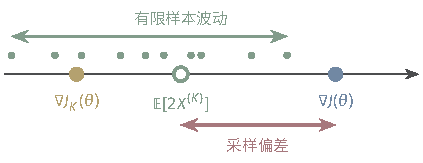
\includegraphics[width=72mm]{figures/07-probability/08-sampling-and-integration/tikz/pgrad-error-split/figure.pdf}
  \caption{图~\ref{fig:pgrad-chain-bias}中$K=5$时的误差分解。蓝点为目标梯度$\nabla J(1)=2$；绿圈为公式$2X$在实际抽样规律下的均值$1.345$，它与蓝点之差是采样偏差；上方绿点为$10$次独立重复中$n=20$个样本平均的取值（固定种子），其散布是有限样本波动；黄点为有限步程序的导数$0.904$。}
  \label{fig:pgrad-error-split}
\end{BookInlineFigure}

\paragraph{步数增加时}

本例中$K\to\infty$时三个量都趋于$2$，因为式~\eqref{eq:pgrad-ar-law}给出了闭式。一般情形下，即使$J_{K}\to J$，也推不出$J_{K}'\to J'$。例如
\[
  J_{K}(\theta)=J(\theta)+\frac{1}{K}\sin(K\theta)
\]
满足$\lvert J_{K}-J\rvert\leq1/K$，但$J_{K}'-J'=\cos(K\theta)$不趋于零。函数值的一致逼近不控制导数。要由程序导数得到目标导数，需要导数本身的收敛，例如$J_{K}'$在$\theta$的某个邻域上一致收敛，这时微积分中关于导数一致收敛的定理保证极限就是$J'$。对实际的MCMC程序，这类结论要用到链对参数的可微依赖与遍历性的定量估计，超出了本卷给定分布计算的范围。

实际计算时，比较稳妥的做法是：用前几节在目标下成立的梯度公式，把链上的样本当作计算这个期望的积分样本，然后按第~\ref{chap:monte-carlo-integration-error}章检查初值偏差、相关性与长期方差。这样，梯度的正确性来自目标下的公式，误差的分析来自积分误差的理论，两者各有依据。

\section{本章小结}
\label{sec:pgrad-summary}

章首的问题是：样本平均$\frac{1}{n}\sum_{i}X_{i}^{2}$里看不到参数，对它求导得到零，可$\mathbb{E}[X^{2}]$明明随$\theta$变化。答案是参数通过样本的来源进入了期望，求梯度时必须把它找出来并计入。本章的做法是先把参数的位置看清，再把期望写成某个固定测度上的积分，参数全部移进被积函数，然后用定理~\ref{thm:pgrad-exchange}的局部Lipschitz控制检查求导能否移进积分。逐点可微不够，图~\ref{fig:pgrad-moving-spike}的移动尖峰就是反例。

三种表示对应三种固定测度的选法，各自利用不同的计算条件，也各有失效的情形。

\begin{BookInlineTable}
  \centering
  \caption{三种梯度表示的比较。}
  \label{tab:pgrad-methods}
  \begin{tabular}{@{}llll@{}}
    \toprule
    & 直接求导 & 重参数化 & 得分函数 \\
    \midrule
    固定的测度 & 抽样分布$P$ & 噪声分布$Q$ & 参考测度$\nu$ \\
    需要计算 & $\nabla_{\bm{\theta}}f_{\bm{\theta}}$ & 生成映射及$\nabla_{x}f_{\bm{\theta}}$ & 得分或$\bm{a}_{\bm{\theta}}$ \\
    对$f$的要求 & 对参数可控 & 沿路径可控 & 可求值即可 \\
    典型失效 & 控制不可积 & 离散选择、跳跃 & 支撑随参数移动 \\
    \bottomrule
  \end{tabular}
\end{BookInlineTable}

直接求导适用于抽样分布固定的情形，梯度就是逐样本导数的平均。重参数化把分布的变化改写成样本点的移动，路径导数由链式法则的两条路组成；函数沿路径跳跃时它看不到跳跃的贡献。得分函数估计对概率权重求导，不需要$f$对$x$可微，离散变量与不连续函数都能处理；但它要求支撑不随参数移动，否则会漏掉边界项。归一化常数未知时，得分是未归一化对数导数减去它的期望，梯度化为函数值与对数导数的协方差，只需目标样本；用独立样本估计时，以样本平均为中心的协方差要除以$n-1$。

无论用哪种表示，都要分开检查两件事：梯度样本的可积性保证估计无偏和一致，二阶矩才保证误差按$n^{-1/2}$缩小。不同表示的方差可以相差很多，没有哪一种在所有问题上更好；得分估计可以借助得分期望为零加入基线，基线若用到当前样本，须像留一基线那样保证与该样本的得分独立。样本来自近似生成器或有限步链时，估计误差分成与样本数无关的采样偏差和有限样本波动；对有限步程序求导得到的是程序期望的导数，它与目标导数是否相同要另行证明。

本章只回答怎样把期望的导数变成可估计的积分，以及这个估计的偏差与波动。用这些梯度逐步更新参数，是随机优化的问题。下一章在共同的精度要求下，比较各种采样、方差控制与梯度表示的计算预算，讨论怎样为具体任务选择方法。

